\documentclass[12pt,letterpaper,twocolumn]{article}

% Fonts and page layout
\usepackage[T1]{fontenc}
\usepackage{lmodern,microtype}
\usepackage[margin=1in]{geometry}

% Mathematics, figures and tables
\usepackage{amsmath,amssymb}
\usepackage{graphicx,booktabs,makecell}
\usepackage{caption,placeins,float}
\usepackage{xcolor,titlesec}
\usepackage[hidelinks]{hyperref}
\usepackage{xurl}
\usepackage{listings}
\lstset{basicstyle=\fontsize{10}{11}\selectfont\ttfamily,
 breaklines=true,breakatwhitespace=false,breakautoindent=true,
 columns=fullflexible,keepspaces=true,
 showstringspaces=false,frame=single,aboveskip=6pt,belowskip=6pt}

% Paragraphs and columns
\setlength{\columnsep}{0.25in}
\setlength{\parindent}{1em}
\setlength{\parskip}{2pt plus 1pt}
\setlength{\emergencystretch}{2em}
\raggedbottom

% Section headings
\titleformat{\section}{\large\bfseries}{\thesection}{0.5em}{}
\titlespacing*{\section}{0pt}{12pt plus 2pt}{5pt}
\titlespacing*{\subsection}{0pt}{9pt plus 2pt}{3pt}
\titlespacing*{\subsubsection}{0pt}{7pt plus 1pt}{2pt}

% Captions and tables
\captionsetup{font=small,labelfont=bf,skip=2pt}
\captionsetup[table]{position=top}
\renewcommand{\arraystretch}{1.05}
\let\originaltabular\tabular
\renewcommand{\tabular}{\small\originaltabular}

% Float placement
\renewcommand{\topfraction}{0.9}
\renewcommand{\bottomfraction}{0.8}
\renewcommand{\textfraction}{0.1}
\renewcommand{\floatpagefraction}{0.7}
\renewcommand{\dbltopfraction}{0.9}
\renewcommand{\dblfloatpagefraction}{0.7}
\setcounter{topnumber}{3}
\setcounter{bottomnumber}{2}
\setcounter{dbltopnumber}{3}
\setlength{\textfloatsep}{10pt plus 2pt minus 2pt}
\setlength{\dbltextfloatsep}{8pt plus 1pt minus 1pt}
\setlength{\floatsep}{8pt}
\setlength{\dblfloatsep}{8pt}
\setlength{\intextsep}{8pt plus 2pt minus 2pt}

% Keep figure pages compact instead of stretching the gaps between floats.
\makeatletter
\setlength{\@fptop}{0pt}
\setlength{\@fpsep}{10pt}
\setlength{\@fpbot}{0pt plus 1fil}
\setlength{\@dblfptop}{0pt}
\setlength{\@dblfpsep}{10pt}
\setlength{\@dblfpbot}{0pt plus 1fil}
\makeatother

% Equation spacing
\AtBeginDocument{%
  \setlength{\abovedisplayskip}{5pt plus 2pt minus 1pt}
  \setlength{\belowdisplayskip}{5pt plus 2pt minus 1pt}
  \setlength{\abovedisplayshortskip}{3pt plus 1pt}
  \setlength{\belowdisplayshortskip}{3pt plus 1pt}
}

% Include figures from the project root
\newcommand{\reportfigure}[2][]{\includegraphics[#1]{#2}}

\AtEndDocument{\clearpage\ifnum\numexpr\value{page}-1\relax>25
\PackageError{report}{Report exceeds the 25-page limit: \thepage\space pages}{Reduce length before submission.}
\fi}
\begin{document}

\twocolumn[{%
  \noindent
  \begin{minipage}[t]{0.64\textwidth}
    \textbf{Group Name: Artemis}\\
    Grace Davis, Navya Agarwal,\\
    Olivia Motkowski, Sarah Schmidt
  \end{minipage}\hfill
  \begin{minipage}[t]{0.34\textwidth}
    \raggedleft
    \textbf{October 21, 2026}\\
    ASTRO 320W
  \end{minipage}

  \vspace{1.5em}
  {\centering\Large\bfseries
    Astro 320W Midterm Observing Report\par}
  \vspace{1em}
}]

\section*{Introduction}
We used the Davey Laboratory 24-inch telescope and CCD camera to
measure read noise, dark signal, flat-field response, and gain.
We then tested stellar focus and photometric repeatability, measured
instrumental colors in M29, made a BVR image of NGC 7129, and
estimated plate scale from visual binaries. The measurements show
how calibration, saturation, and observing conditions affect CCD
photometry.

\section{Exercise A: CCD Characteristics}
Digital number (DN) and analog-to-digital unit (ADU) refer to the same
signal unit. Unless stated otherwise, regional measurements in this
exercise use a central $100\times100$-pixel square with zero-based
upper-left coordinates $(1478,1478)$ in the unbinned
$3056\times3056$-pixel images.

\subsection{Bias Frames and Read Noise}
We used two instructor-provided Python scripts,
\nolinkurl{A320_bf_stdev_final.ipynb} and
\nolinkurl{A320_bf_stdev_ROI.ipynb}, to measure temporal read noise
from 20 raw bias frames. The first script evaluates the full detector;
the second evaluates a user-selected square region. Both calculate
each pixel's standard deviation across the bias stack, then average
those standard deviations over the selected pixels:
\begin{equation}
\sigma_t(x,y)=\sqrt{\frac{1}{N}\sum_{i=1}^{N}
[B_i(x,y)-\overline{B}(x,y)]^2}.
\end{equation}
With population normalization ($N=20$, $\mathrm{ddof}=0$), the
full-detector result was 9.645 DN; sample normalization gives
9.896 DN. This method excludes stable pixel-to-pixel bias structure.
The earlier random region was not recorded, so regional comparisons
use the central square defined above.

The remaining Exercise A measurements were made in AstroImageJ,
with calculations and plotting in Excel. We formed a master bias
by averaging the 20 frames with AstroImageJ's
Average Intensity projection after conversion to 32-bit. Subtracting
this master from each input frame reduced the mean spatial standard
deviation from 13.847 to 9.790 DN (Table~\ref{tab:a_bias_statistics}).

\begin{table*}[tp]
 \centering
 \caption{Full-image spatial standard deviations from 20 bias frames.
 Sample SD describes scatter among the measured standard deviations.
 Nominal SEM is sample SD divided by $\sqrt{20}$. The corrected
 measurements share a master bias and are not independent.}
 \label{tab:a_bias_statistics}
 \begin{tabular}{lrrr}
  \toprule
  Images & Mean spatial SD (DN) & Sample SD (DN) & Nominal SEM (DN)\\
  \midrule
  Raw bias frames & 13.847 & 0.092 & 0.021\\
  Bias-subtracted frames & 9.790 & 0.027 & 0.006\\
  \bottomrule
 \end{tabular}
\end{table*}

The reduction indicates removal of fixed spatial bias structure.
Because each input frame also contributed to the master, the residual
noise is slightly suppressed. For independent input frames with equal
variance,
\begin{equation}
\operatorname{Var}(B_i-\overline{B})=
\sigma_{\mathrm{RN}}^2\left(1-\frac{1}{N}\right).
\end{equation}
The shared-master residuals are therefore not independent read-noise estimates.

\subsubsection{Paired-Bias Measurement}
We also subtracted ten disjoint pairs of raw bias frames (1--2, 3--4,
through 19--20), using 32-bit arithmetic. Subtraction removes stable
bias structure while adding the independent noise variances:
\begin{equation}
\sigma_{\mathrm{diff}}^2=2\sigma_{\mathrm{RN}}^2,
\qquad R_{\mathrm{DN}}=\frac{\sigma_{\mathrm{diff}}}{\sqrt{2}}.
\end{equation}
Table~\ref{tab:a_bias_pairs} gives the full-detector and central-region
measurements.

\begin{table*}[tp]
 \centering
 \caption{Raw-bias pair differences and inferred read noise.
 Central measurements use the same $100\times100$ pixels.
 All values are in DN. The last three central entries are not assigned
 to specific pairs because their export does not preserve pair labels.}
 \label{tab:a_bias_pairs}
 \begin{tabular}{lrrrr}
  \toprule
  Pair & Full $\sigma_{\rm diff}$ & Central $\sigma_{\rm diff}$
       & Full $R$ & Central $R$\\
  \midrule
  1--2   & 14.211 & 14.187 & 10.049 & 10.031\\
  3--4   & 14.199 & 14.058 & 10.040 & 9.940\\
  5--6   & 14.267 & 14.243 & 10.088 & 10.071\\
  7--8   & 14.173 & 14.100 & 10.022 & 9.970\\
  9--10  & 14.209 & 14.209 & 10.047 & 10.047\\
  11--12 & 14.193 & 14.263 & 10.036 & 10.086\\
  13--14 & 14.173 & 14.141 & 10.022 & 9.999\\
  15--16 & 14.245 & --- & 10.073 & ---\\
  17--18 & 14.190 & --- & 10.034 & ---\\
  19--20 & 14.197 & --- & 10.039 & ---\\
  \bottomrule
 \end{tabular}
\end{table*}

The remaining three central difference SDs are 14.286, 14.324, and
14.246 DN in export order; their individual pair assignments need
confirmation. All ten central measurements are included in the mean.
The mean paired estimates were
\begin{equation}
\boxed{R_{\mathrm{full}}=10.045\pm0.007~\mathrm{DN}}
\end{equation}
\begin{equation}
\boxed{R_{\mathrm{central}}=10.045\pm0.019~\mathrm{DN}}
\end{equation}
The uncertainties are SEMs of ten estimates; the sample SDs are
0.021 DN for the full detector and 0.060 DN for the central region.
The smaller region has more scatter, but both means agree.
The full-detector estimate predicts a shared-master residual of
$10.045\sqrt{19/20}=9.791$ DN, matching the measured 9.790 DN.
Small differences from the temporal result are expected because
one method averages pixelwise SDs and the other measures spatial
scatter in difference images.

\subsection{Conversion to Electrons}
The gain measured in Exercise B applies to $2\times2$ binning.
For the $1\times1$ bias and dark images, we instead used the nominal
header value $g_{\mathrm{hdr}}=1.34~\mathrm{e^-\,DN^{-1}}$.
Using $R_{\mathrm{e^-}}=g_{\mathrm{hdr}}R_{\mathrm{DN}}$ gives
\begin{equation}
\boxed{R_{\mathrm{e^-},\mathrm{nom}}=13.46~\mathrm{e^-\,pix^{-1}\,read^{-1}}}.
\end{equation}
The read-noise SEM contributes 0.009 electron; the unknown gain
error is not included.

\subsection{Dark Signal versus Exposure Time}
We measured six dark frames with exposures of 0.1, 6, 10, 30, 45,
and 60 s at a reported cooler setpoint of $0^\circ$C. Actual detector
temperatures were not recorded. We treated the frames as uncorrected because their headers contain
neither \texttt{CALSTAT} nor \texttt{PEDESTAL}.

The central master-bias mean was 1038.930 DN. We calculated net
signal, nominal accumulated charge, and nominal current per pixel as
\begin{align}
D_{\mathrm{net}}&=D_{\mathrm{raw}}-B,\\
Q_{\mathrm{nom}}&=g_{\mathrm{hdr}}D_{\mathrm{net}},\\
I_{\mathrm{nom}}&=Q_{\mathrm{nom}}/t.
\end{align}
The master-bias header records a $-30^\circ$C cooler setpoint,
without a recorded actual CCD temperature. A temperature-dependent
bias offset may therefore remain. The observing notes also record an uncovered
telescope, allowing possible stray-light contamination.

\begin{table*}[tp]
 \centering
 \caption{Central-region dark measurements versus exposure time.
 Electron quantities use the nominal gain of
 $1.34~\mathrm{e^-\,DN^{-1}}$. Individual measurement errors are unavailable.}
 \label{tab:a_dark_time}
 \begin{tabular}{rrrr}
  \toprule
  $t$ (s) & Net signal (DN) &
  $Q_{\rm nom}$ ($\mathrm{e^-\,pix^{-1}}$) &
  $I_{\rm nom}$
  ($\mathrm{e^-\,pix^{-1}\,s^{-1}}$)\\
  \midrule
  0.1 & 31.568 &
  $42.30$ &
  $423.02$\\
  6 & 58.079 &
  $77.83$ &
  $12.97$\\
  10 & 113.585 &
  $152.20$ &
  $15.22$\\
  30 & 279.962 &
  $375.15$ &
  $12.50$\\
  45 & 452.548 &
  $606.41$ &
  $13.48$\\
  60 & 654.913 &
  $877.58$ &
  $14.63$\\
  \bottomrule
 \end{tabular}
\end{table*}

The 0.1-s frame gives a much higher apparent rate than the longer
exposures. Dividing an additive offset by a short exposure can produce
this behavior. We retained the point in the table and plot but excluded
it from the time-trend fit.

For the five 6--60-s rates, the arithmetic mean was
\begin{equation}
\boxed{\overline{I}_{\mathrm{nom}}=13.76\pm0.51~
\mathrm{e^-\,pix^{-1}\,s^{-1}}}.
\end{equation}
The sample SD was $1.14~\mathrm{e^-\,pixel^{-1}\,s^{-1}}$;
the quoted uncertainty is its SEM, assuming independent measurements.
An unweighted fit $Q_{\mathrm{nom}}=mt+b$ gave
\begin{align}
m&=14.33\pm0.78~\mathrm{e^-\,pixel^{-1}\,s^{-1}},\\
b&=-14.8\pm28.4~\mathrm{e^-\,pixel^{-1}}.
\end{align}
These fit errors come from the residual scatter. The approximately
linear charge increase and intercept consistent with zero support a
roughly constant accumulation rate over 6--60 s. Bias mismatch,
uncertain temperature, and stray light prevent attributing the entire
signal to intrinsic dark current.

\begin{figure*}[htbp]
 \centering
 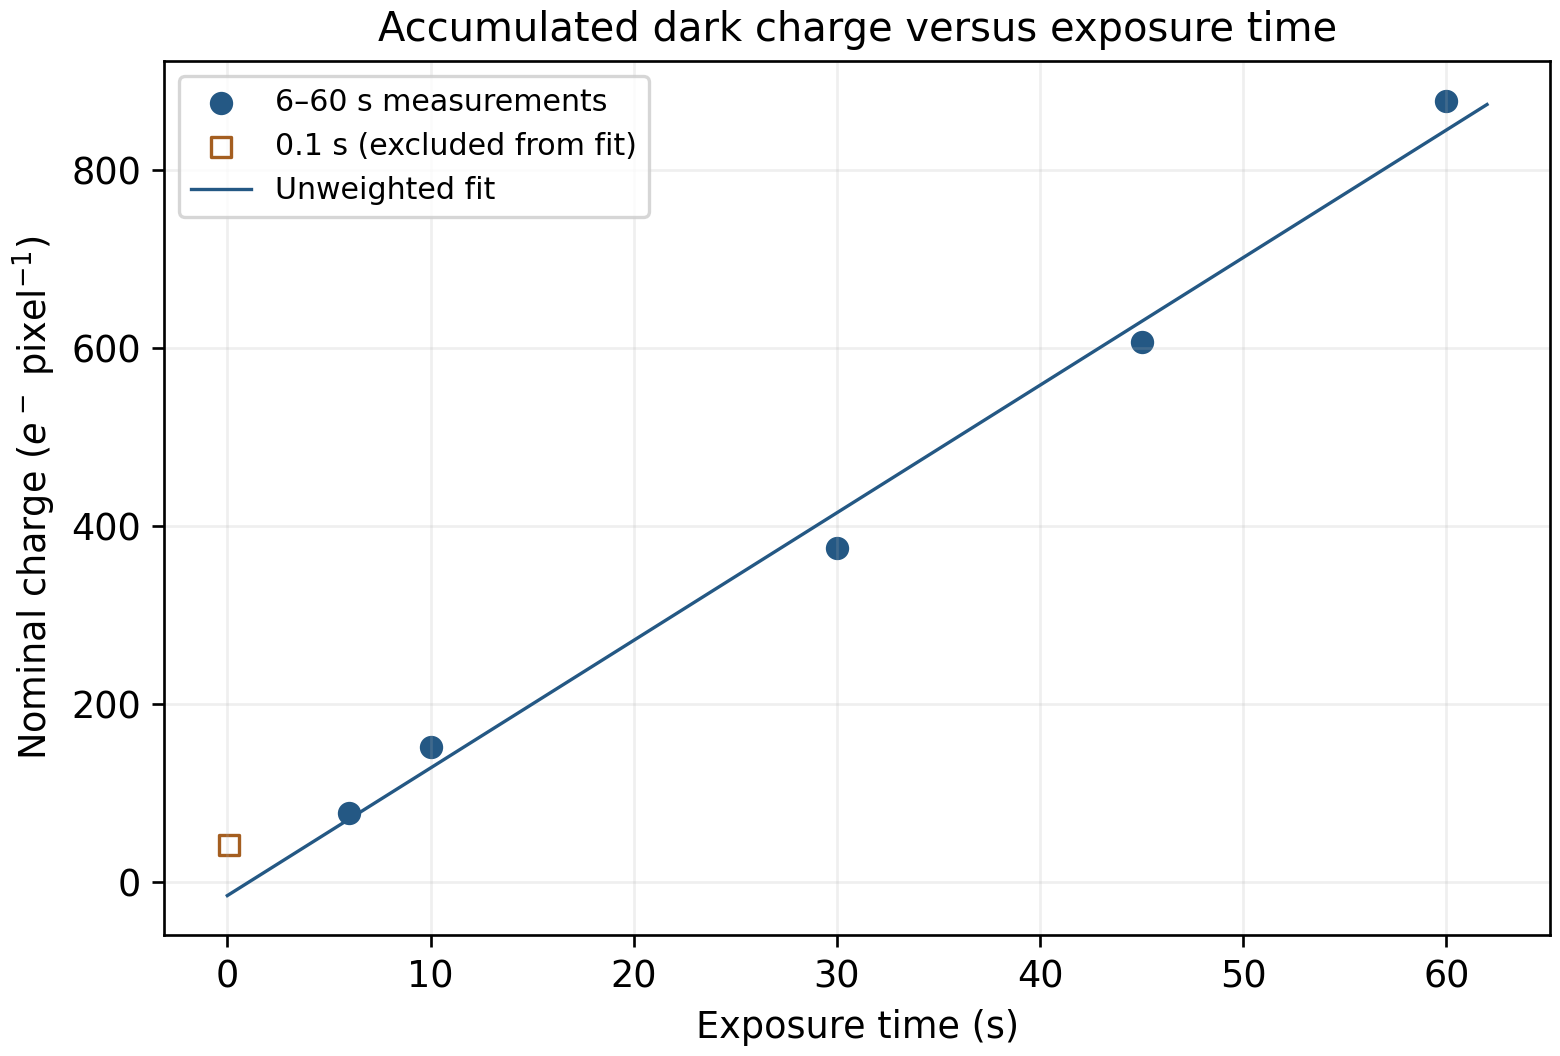
\includegraphics[width=0.8\textwidth]{01_dark_charge_vs_time.png}
 \caption{Accumulated nominal dark charge versus exposure time.
 The unweighted fit uses the five 6--60-s frames; individual
 measurement errors are unavailable.
 The 0.1-s point is shown but excluded from the fit.
 The reported cooler setpoint was $0^\circ$C; actual CCD
 temperatures are unavailable.}
 \label{fig:a_dark_charge_time}
\end{figure*}

\subsection{Temperature Dependence}
Four temperature-series files have verified 300-s exposures and
recorded starting CCD temperatures (Table~\ref{tab:a_dark_temperature}).
The observing sequence was interrupted, and labeling problems left no
identifiable, usable 300-s observations at the intended $-20^\circ$C
and $-25^\circ$C settings. We therefore restricted the analysis to the
four verified frames; the coldest retained starting temperature was
$-7.844^\circ$C. This reduced temperature range limits the thermal fit.

We used the recorded starting temperatures rather than the filenames,
and applied the same central region, master bias, and nominal gain
as in the exposure-time analysis.

\begin{table*}[tp]
 \centering
 \caption{Verified temperature-series observations.
 All exposures are 300 s. Starting temperatures differ from the cooler setpoints.}
 \label{tab:a_dark_temperature}
 \begin{tabular}{lrrrr}
  \toprule
  File & Setpoint ($^\circ$C) & Start ($^\circ$C) &
  Raw mean (DN) &
  $I_{\rm nom}$
  ($\mathrm{e^-\,pix^{-1}\,s^{-1}}$)\\
  \midrule
  \texttt{-10C.fit} & $-10$ & $-7.844$ & 1048.4342 &
  $0.042$\\
  \texttt{0C.fit} & 0 & 0.844 & 1092.8636 &
  $0.241$\\
  \texttt{10C.fit} & 10 & 18.750 & 1338.7558 &
  $1.339$\\
  \texttt{20C.fit} & 26 & 20.219 & 1922.2905 &
  $3.946$\\
  \bottomrule
 \end{tabular}
\end{table*}

Individual error bars are omitted because the per-image uncertainty
method is undocumented. The reported SEM and regression errors
exclude shared bias and gain errors; temperature and timing errors
were unavailable.

\begin{figure*}[htbp]
 \centering
 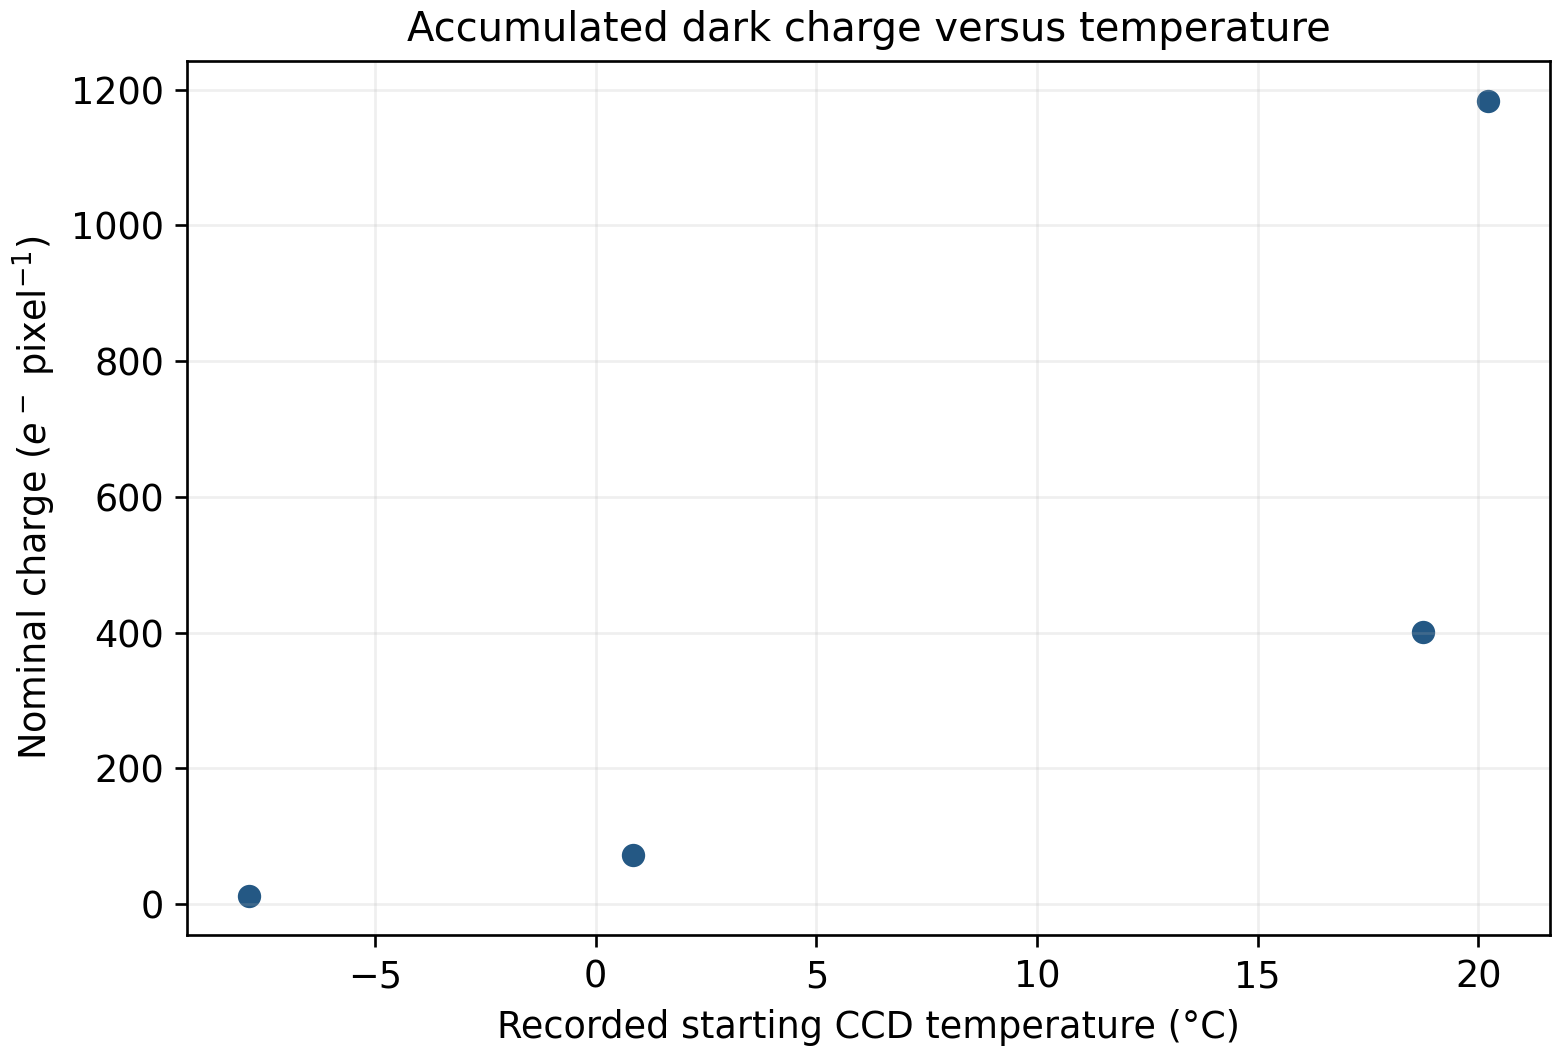
\includegraphics[width=0.8\textwidth]{02_dark_charge_vs_temperature.png}
 \caption{Accumulated nominal dark charge versus recorded starting
 CCD temperature for four 300-s observations.
 Individual error bars are omitted. Bias-temperature mismatch,
 gain uncertainty, and unknown temperature history limit interpretation.}
 \label{fig:a_dark_charge_temperature}
\end{figure*}

Current rises with recorded temperature, although the two warmest
frames have similar starting temperatures and markedly different
rates. Their temperatures may have changed during exposure; starting
temperatures alone do not establish thermal equilibrium. The coldest
net signal is also particularly sensitive to bias subtraction.

\subsubsection{Apparent Activation Energy}
We tested the simple thermal model
\begin{equation}
I(T)=I_0\exp\left(-\frac{A}{kT}\right),
\end{equation}
where $T=T_{\mathrm{start}}+273.15$ K and
$k=8.617333\times10^{-5}~\mathrm{eV\,K^{-1}}$.
Taking a dimensionless logarithm gives
\begin{equation}
\ln\left(\frac{I}{I_{\mathrm{ref}}}\right)
=c-\frac{A}{k}\frac{1}{T},
\end{equation}
with $I_{\mathrm{ref}}=1~\mathrm{e^-\,pixel^{-1}\,s^{-1}}$.
An unweighted fit to the four points gave a slope
$m_T\simeq-1.107\times10^4$ K and
\begin{equation}
\boxed{A_{\mathrm{app}}=-km_T=0.95\pm0.14~\mathrm{eV}}.
\end{equation}
The uncertainty follows from the regression slope error,
$\sigma_A=k\sigma_{m_T}$.

\begin{figure*}[htbp]
 \centering
 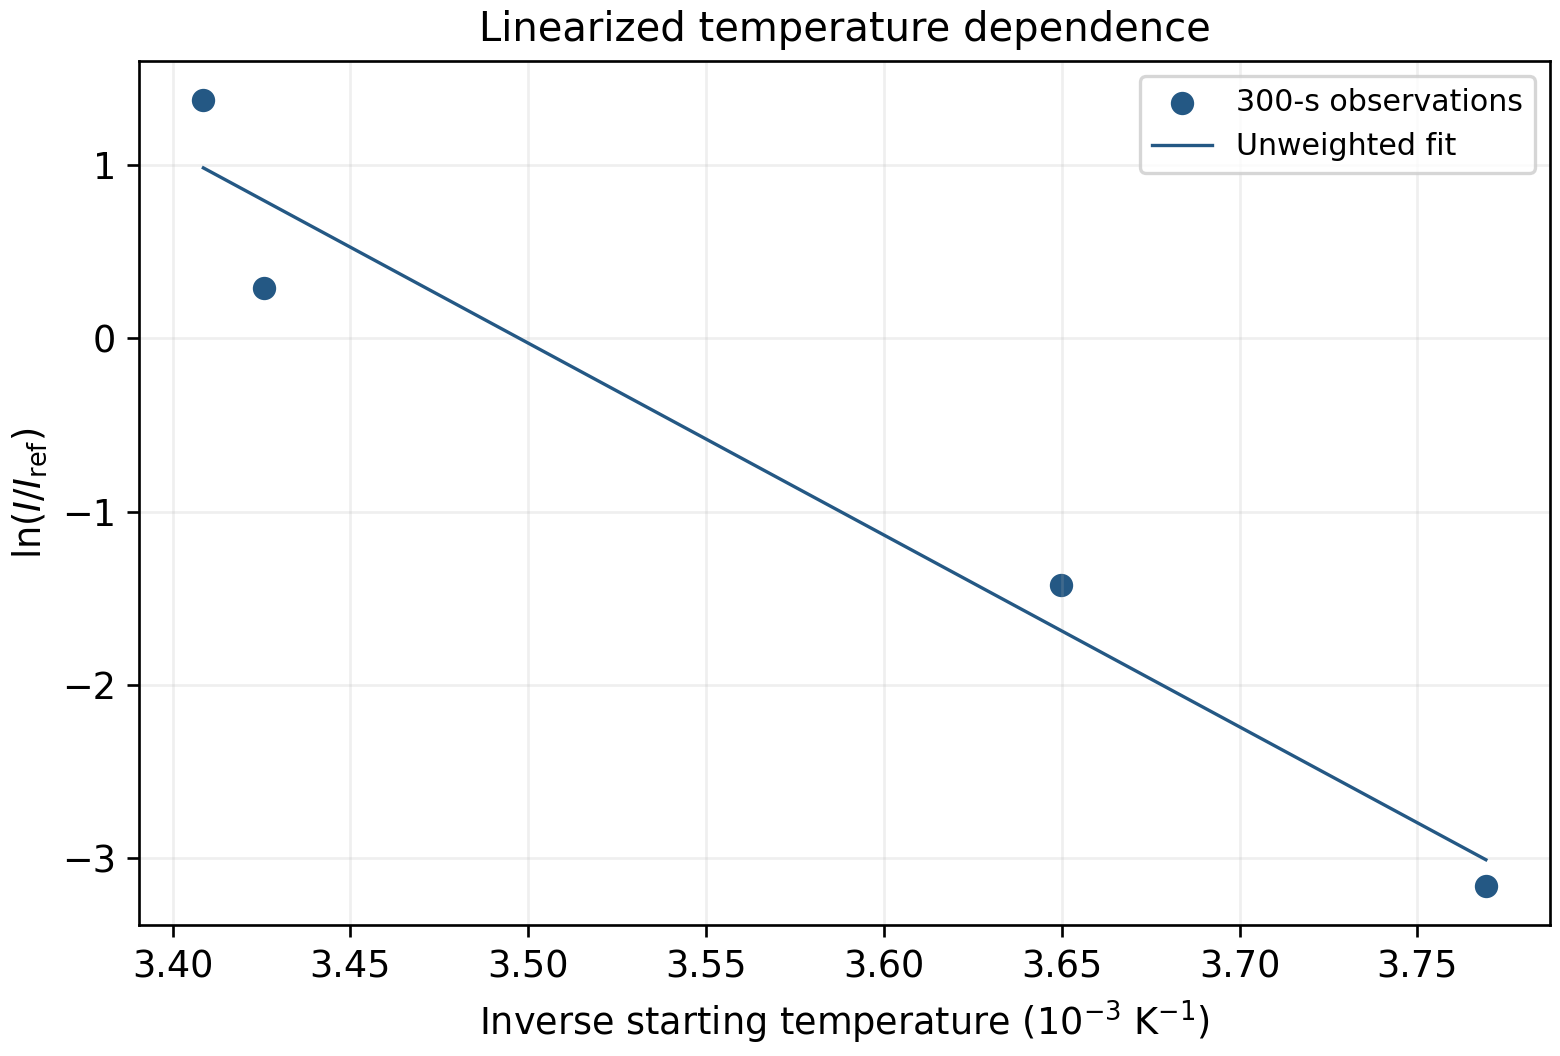
\includegraphics[width=0.8\textwidth]{03_linearized_thermal_fit.png}
 \caption{Linearized temperature dependence for the four verified
 300-s frames. Individual error bars are omitted.
 The line is an unweighted fit; the
 activation-energy uncertainty comes from regression residuals.}
 \label{fig:a_thermal_fit}
\end{figure*}

The rise with temperature is consistent with thermal generation,
but the unmatched bias and uncertain temperature histories limit
this activation-energy estimate. Additive bias errors and incorrect
temperatures can change the fitted slope.

% Allow pending figures to flow across exercise boundaries.
\section{Exercise B: Flat Fields and Gain}
\subsection{Photon Transfer Curves}
We measured regional mean signals and spatial SDs with AstroImageJ
and made the original PTCs in Excel. The region coordinates were not
saved. Figures~\ref{fig:sky_ptc} and \ref{fig:dome_ptc} replot these
results with tighter logarithmic axes.

The dome sequence contains 13 frames at seven exposures: 6, 12, 15,
18, 30, 45, and 90 s. Lamp settings also changed. The headers record
acquisition-time dark subtraction (\texttt{CALSTAT=D}) and
\texttt{PEDESTAL=-100}; whether that offset was removed for the
original PTC is unrecorded. Individual plotted points have not been
matched to filenames.

The sky sequence contains twenty 6-s R-band images. The measured
regions have means of 16048--38285 DN and maxima of 26013--47914 DN.
The first frame contains three pixels at 65535 DN outside the
measured region; the other 19 frames have no digitally clipped pixels.
The sampled regions are unclipped, but the full set is not entirely
unsaturated. Prior dark correction is not established by the headers.

For a photon-dominated, offset-corrected signal $S$,
\begin{equation}
\sigma^2\simeq S/g,\qquad \sigma\propto\sqrt{S}.
\end{equation}
The expected log--log noise--signal slope is therefore $1/2$.
The sky curve rises with signal; the dome curve rises before turning
over at high signal. These are qualitative observations, since flat
spatial variance also contains illumination gradients and sensitivity
structure. We did not fit a numerical slope to these curves.

\begin{figure*}[tp]

  \centering
  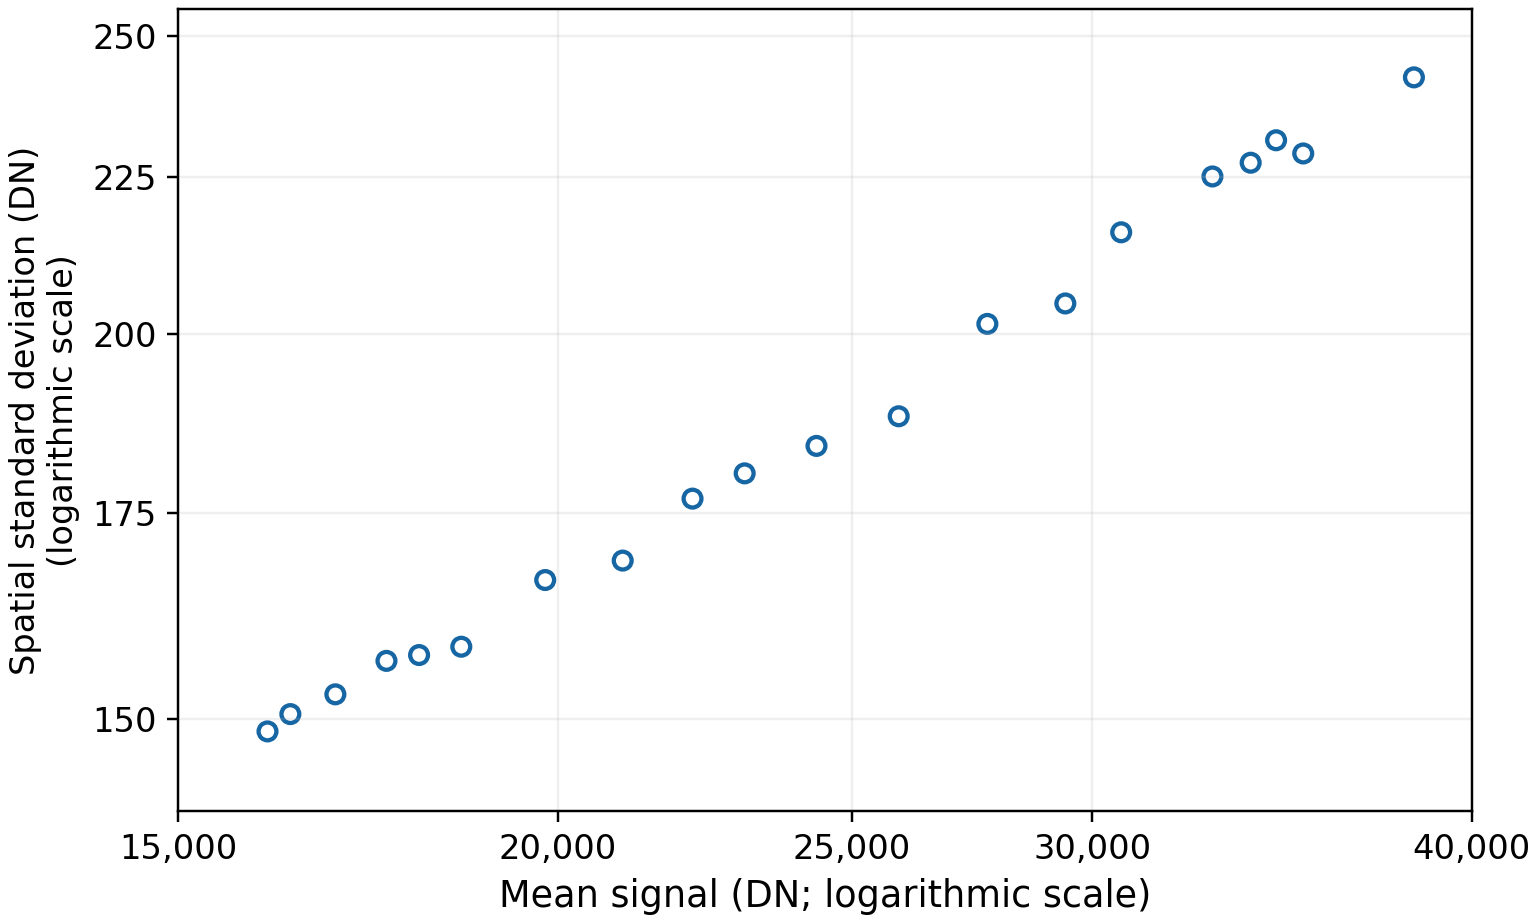
\includegraphics[width=0.8\textwidth]{sky_flat_PTC.png}
 \caption{Sky-flat photon transfer curve replotted from the 20 original
  AstroImageJ measurements. Both axes are logarithmic; the vertical
  range is restricted to 140--255 DN to show the trend clearly.
  Regional spatial standard deviation is plotted against mean signal.}
  \label{fig:sky_ptc}
 
\end{figure*}

\begin{figure*}[tp]

  \centering
  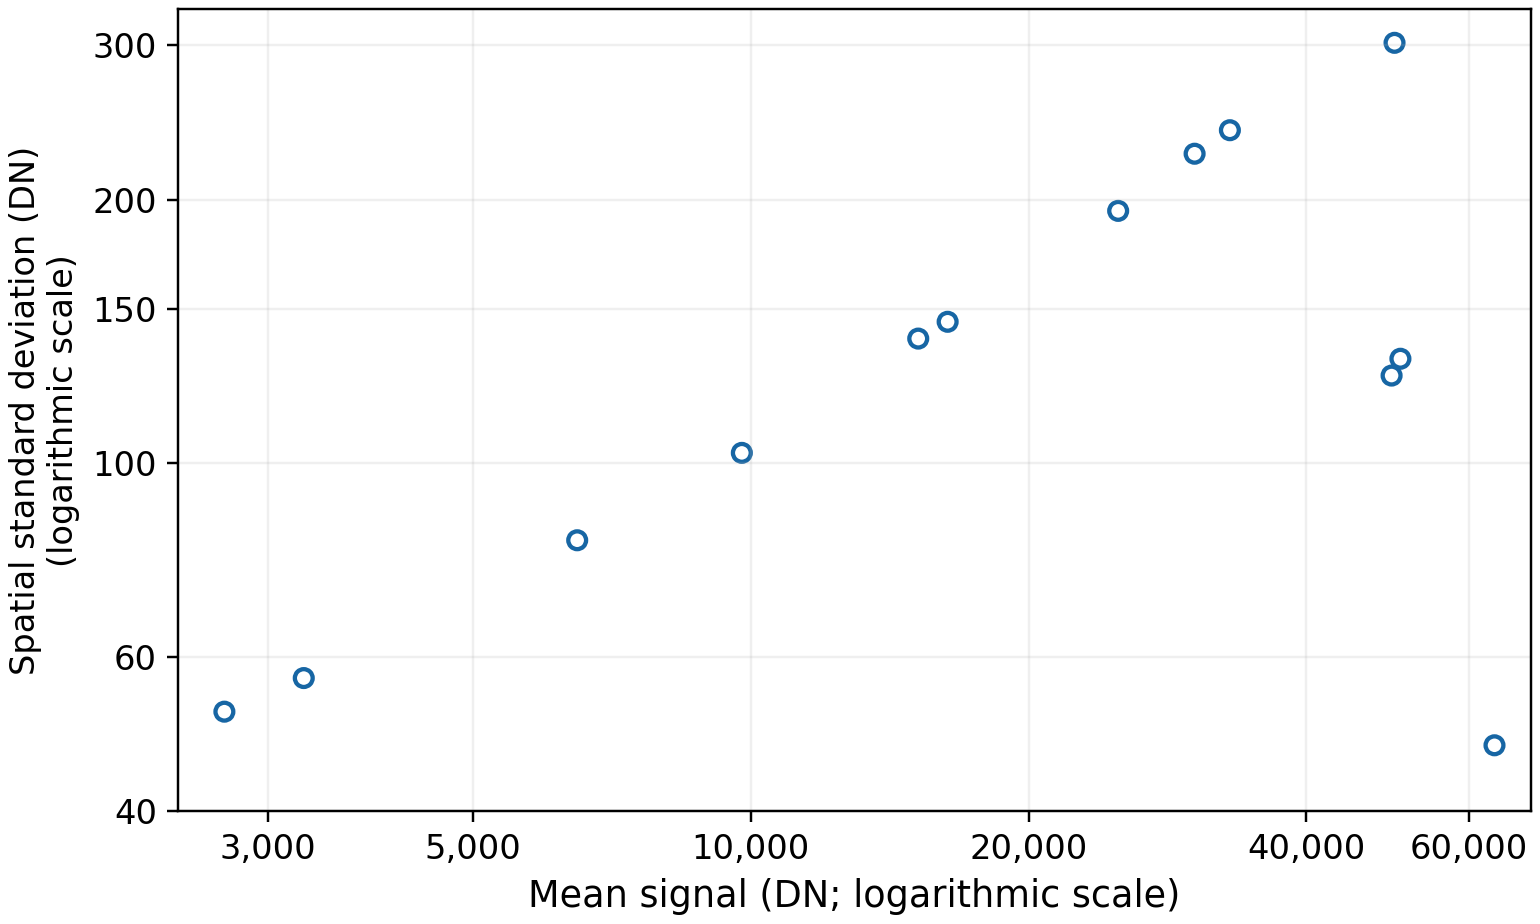
\includegraphics[width=0.8\textwidth]{Dome Flat Photon Transfer Curve.png}
 \caption{Dome-flat photon transfer curve with tightened log--log axes.
  Points are approximately digitized from the preserved AstroImageJ
  plot; the original numerical export is unavailable. Noise rises
  before turning over at high signal. No fit uses the digitized values.}
  \label{fig:dome_ptc}
 
\end{figure*}

\subsection{Gain from Paired Dome Flats}
\label{sec:b_gain}
We measured gain from a separate set of twenty 0.2-s and twenty 10-s
dome flats, all binned $2\times2$ ($1528\times1528$ pixels).
These images were dark-corrected during acquisition. A comparison of
stored and displayed values showed that their 100-DN pedestal remained
in AstroImageJ, so we converted the images to 32-bit and subtracted
100 DN once, without another dark or bias subtraction.

We formed ten disjoint pairs at each duration and measured the two
means and the difference-image standard deviation in a central
$100\times100$-pixel region starting at $(714,714)$. No alignment,
smoothing, or normalization was applied. The first 10-s pair was recorded in Excel; the 0.2-s pairs used
\nolinkurl{Measure_0p2s_Dome_Gain.ijm}.
In the photon-only approximation,
\begin{equation}
g_{\mathrm{ph}}=
\frac{\overline{F}_1+\overline{F}_2}{\sigma_{F_1-F_2}^2}.
\end{equation}
In the 10-s measurement workbook, means of 27292.439 and
27332.640 DN and a difference SD of 206.305 DN give $1.283~\mathrm{e^-\,DN^{-1}}$.

\begin{table}[htbp]
 \centering
 \caption{Photon-only paired-flat gain estimates, in
 $\mathrm{e^-\,DN^{-1}}$.
 This estimator does not remove read noise.}
 \label{tab:b_gain_pairs}
 \begin{tabular}{lrr}
  \toprule
  Pair & 0.2-s flats & 10-s flats\\
  \midrule
  1--2   & 0.836 & 1.283\\
  3--4   & 0.804 & 1.274\\
  5--6   & 0.836 & 1.264\\
  7--8   & 0.854 & 1.232\\
  9--10  & 0.810 & 1.280\\
  11--12 & 0.834 & 1.271\\
  13--14 & 0.825 & 1.294\\
  15--16 & 0.831 & 1.289\\
  17--18 & 0.828 & 1.296\\
  19--20 & 0.837 & 1.270\\
  \bottomrule
 \end{tabular}
\end{table}

The 10-s estimates average $1.275~\mathrm{e^-\,DN^{-1}}$
(sample SD 0.019; SEM 0.006). The 0.2-s estimates average
$0.829~\mathrm{e^-\,DN^{-1}}$ (sample SD 0.014; SEM 0.005).
Additive noise increases the variance relative to photon signal,
which can bias the low-signal estimate downward without a change
in physical gain.

To allow an additive variance term, we fitted
\begin{align}
S&=(\overline{F}_1+\overline{F}_2)/2,\\
V&=\sigma_{F_1-F_2}^2/2=aS+c,\qquad g=1/a.
\end{align}
An unweighted fit to all twenty pairs gave $a\simeq0.7751$,
$c\simeq251~\mathrm{DN^2}$, and
\begin{equation}
\boxed{g_{2\times2}=1.290\pm0.006~\mathrm{e^-\,DN^{-1}}}.
\end{equation}
The gain uncertainty is the fitted slope error propagated as
$\sigma_g=\sigma_a/a^2$. The intercept includes read noise and
possible acquisition-calibration noise or residual offsets.
Since the pairs occupy only two main signal levels, intermediate
exposures would provide a better linearity test.

\subsection{Illumination Profiles and Flat-Field Comparison}
We measured approximately central horizontal and vertical profiles
with AstroImageJ's line-profile tool. In the sky flat, the horizontal
signal rises from about $2.6\times10^4$ DN to
$3.4$--$3.45\times10^4$ DN before falling toward the opposite edge.
The vertical profile runs from about $3.35\times10^4$ DN through a
maximum of $3.46\times10^4$ DN to $3.23\times10^4$ DN.

\begin{figure*}[tp]
\centering
\begin{minipage}[t]{0.48\textwidth}
\centering
  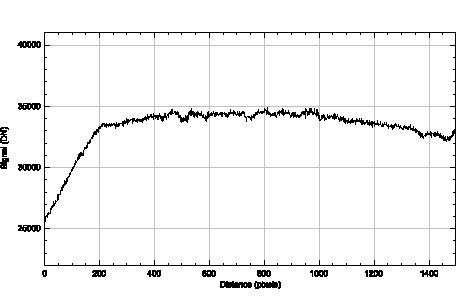
\includegraphics[width=\linewidth,height=0.23\textheight,keepaspectratio]{sky_flat_horizontal_profile.pdf}
 \caption{Horizontal illumination profile through a sky flat.}
  \label{fig:sky_horizontal}
\end{minipage}
\hfill
\begin{minipage}[t]{0.48\textwidth}
\centering
  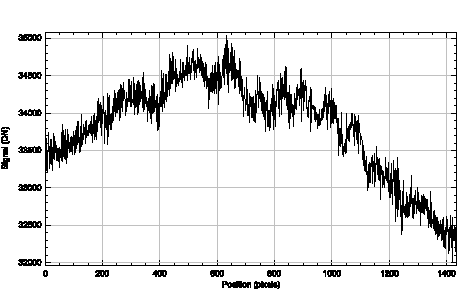
\includegraphics[width=\linewidth,height=0.23\textheight,keepaspectratio]{sky_flat_vertical_profile.pdf}
 \caption{Vertical illumination profile through a sky flat.}
  \label{fig:sky_vertical}
\end{minipage}

\vspace{6pt}

\begin{minipage}[t]{0.48\textwidth}
\centering
  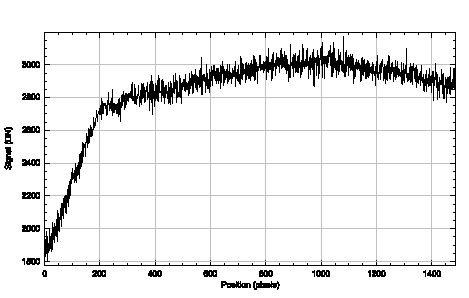
\includegraphics[width=\linewidth,height=0.23\textheight,keepaspectratio]{dome_flat_horizontal_profile.pdf}
 \caption{Horizontal illumination profile through a dome flat.}
  \label{fig:dome_horizontal}
\end{minipage}
\hfill
\begin{minipage}[t]{0.48\textwidth}
\centering
  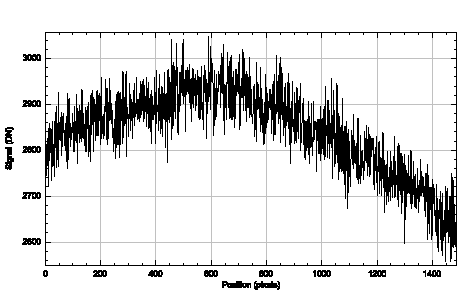
\includegraphics[width=\linewidth,height=0.23\textheight,keepaspectratio]{dome_flat_vertical_profile.pdf}
 \caption{Vertical illumination profile through a dome flat.}
  \label{fig:dome_vertical}
\end{minipage}
\end{figure*}

In the dome flat, the horizontal signal rises from about
$1.85\times10^3$ to $3.0\times10^3$ DN, a 62\% increase relative
to the darker edge. The vertical profile rises from
$2.82\times10^3$ DN to $2.94$--$2.96\times10^3$ DN, then falls
to $2.63\times10^3$ DN.

Both flats show gradients from illumination, vignetting, or detector
response. Their different brightnesses require normalization before
a quantitative comparison of profile shapes.

Sky flats reproduce the science light path more closely, but twilight
limits the observing window and introduces changing brightness,
stars, and sky gradients. Dome flats offer controlled illumination
and can be collected after dark, but the screen may illuminate the
optics differently from the sky. Neither flat type is automatically
free of large-scale gradients.

The representative flats in Figure~\ref{fig:flat_examples} share
ring-shaped shadows and a dark region near the right edge, suggesting
structure in the optical path. Separate display ranges emphasize
these features.

\begin{figure*}[tp]
\centering
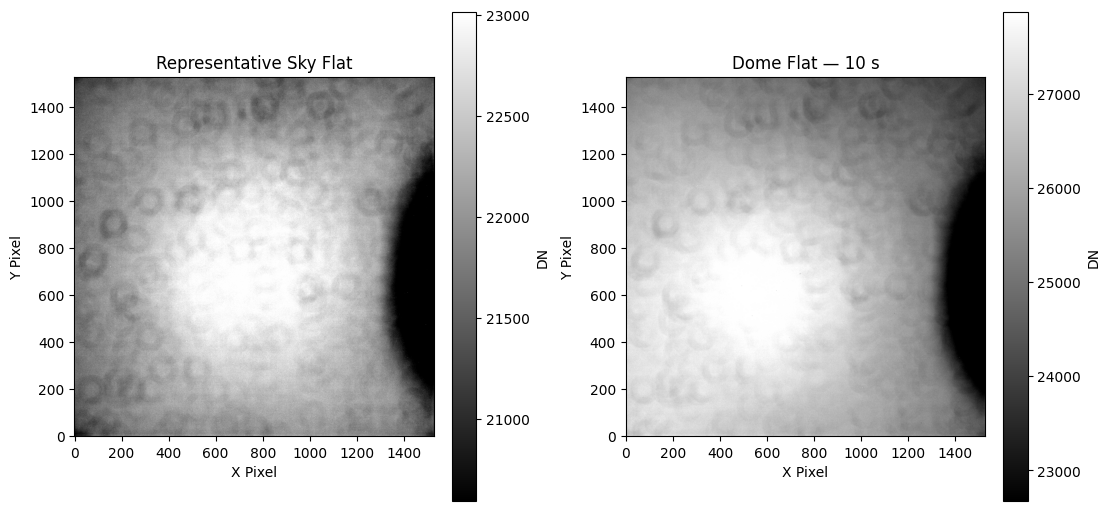
\includegraphics[width=\textwidth]{sky_dome_images.png}
\caption{Representative sky flat and 10-s dome flat. Separate DN
scales emphasize spatial structure. The profile frames were not individually identified.}
\label{fig:flat_examples}
\end{figure*}

\subsection{Saturation}
A pixel signal can saturate at the CCD full well, in the analog
electronics, or at the ADC. The 16-bit digital ceiling is
$2^{16}-1=65535$ DN. Table~\ref{tab:saturation} lists preserved
high-signal dome measurements; their exact input files and offset
handling were not recorded.

\begin{table*}[tp]
 \centering
 \caption{Original high-signal dome-flat measurements used to
 investigate saturation.}
 \label{tab:saturation}
 \begin{tabular}{rrrr}
  \toprule
  Mean (DN) & StdDev (DN) & Min (DN) & Max (DN)\\
  \midrule
  49683.201 & 138.673 & 41776 & 49785\\
  51474.074 & 152.154 & 46572 & 53144\\
  64376.194 & 63.203 & 60650 & 64457\\
  \bottomrule
 \end{tabular}
\end{table*}

At a mean of about $6.44\times10^4$ DN, the spatial SD drops to
about 63 DN. This turnover indicates a nonlinear or clipped response.
The maximum near $6.45\times10^4$ DN is close to the digital ceiling,
but calibration offsets complicate that comparison. The FITS headers identify the camera as an SBIG STX-9000.
Its manufacturer specifies a KAF-09000 sensor, a nominal
$110000~\mathrm{e^-}$ full well, and a 16-bit ADC \cite{camera}.
At the measured binned gain, the full digital range represents about
\begin{equation}
g_{2\times2}(65535)\simeq8.45\times10^4~\mathrm{e^-}.
\end{equation}
This is below even the nominal single-pixel full-well capacity,
supporting the ADC as the expected limit before the photopixel well
fills, provided the analog electronics remain linear. The observed
turnover near the digital ceiling is consistent with that ordering.
However, binning, electronic headroom, and calibration offsets affect
the recorded threshold. Our measurements do not independently exclude
an earlier analog limit or measure the full-well capacity.

\subsection{Uncertainties}
Spatial SD includes illumination gradients and sensitivity structure
as well as photon and read noise. The PTCs provide no errors on the
SDs. The gain-fit uncertainty excludes missing calibration records
and any systematic error from the selected region.

% Allow pending figures to flow across exercise boundaries.
\section{Exercise C: Stellar Image Quality and Photometry}
\subsection{Observations and Calibration}
We observed Omicron Aquilae (54 Aql) for the focus sequence and Ogma
(HD 149026) for repeatability and exposure-time tests, using the
24-inch telescope and Johnson R filter. Wind disturbed the pointing,
with reported errors reaching about 5 arcseconds. All 15 repeatability images have $2\times2$ binning and
$1528\times1528$ pixels.

We calibrated the Exercise C images by subtracting a master dark,
which already included the bias signal, and dividing by the normalized
R-band dome flat:
\begin{equation}
I_{\mathrm{cal}}=
\frac{I_{\mathrm{raw}}-D_{\mathrm{master}}}{F_{\mathrm{normalized}}}.
\end{equation}
Calibration, FWHM measurements, and aperture photometry used
AstroImageJ. No separate bias was subtracted. Python calculated
statistics and made plots from the exports. Repeatability used
individual images, not the aligned median stacks made for display.

\subsection{Focus}
The focus sequence used 6-s exposures with $2\times2$ binning,
starting at $17000~\mu\mathrm{m}$ and decreasing in
$500~\mu\mathrm{m}$ steps. We measured FWHM in AstroImageJ as the
profile width halfway between the local background and peak.

\begin{table}[htbp]
 \centering
 \caption{AstroImageJ FWHM measurements of Omicron Aquilae
 at different focus positions.}
 \label{tab:focus_measurements}
 \begin{tabular}{crr}
  \toprule
  CCD Image & Focus ($\mu$m) & FWHM (pixels)\\
  \midrule
  1 & 17000 & 11.55\\
  2 & 17000 & 12.41\\
  3 & 17000 & 11.19\\
  4 & 16500 & 10.30\\
  6 & 16000 & 9.75\\
  7 & 16000 & 10.68\\
  8 & 15500 & 10.72\\
  9 & 15000 & 12.74\\
  \bottomrule
 \end{tabular}
\end{table}

\begin{figure*}[tp]
\centering
\begin{minipage}[t]{0.48\textwidth}
\centering
 \reportfigure[width=\linewidth,height=0.23\textheight,keepaspectratio]{fwhm_vs_focus.pdf}
 \caption{Omicron Aquilae FWHM versus focus. Blue: individual measurements;
 orange: repeated-position means with sample-SD bars.
 The dashed quadratic shows the focus trend.}
 \label{fig:focus}
\end{minipage}
\hfill
\begin{minipage}[t]{0.48\textwidth}
\centering
  \reportfigure[width=\linewidth,height=0.23\textheight,keepaspectratio]{ogma_repeatability.pdf}
 \caption{Count rates from fifteen 8-s Ogma exposures.
  The line marks the mean; bars are formal AstroImageJ
  count errors divided by exposure time.}
  \label{fig:repeatability}
\end{minipage}

\vspace{6pt}

\begin{minipage}[t]{0.48\textwidth}
\centering
  \reportfigure[width=\linewidth,height=0.23\textheight,keepaspectratio]{ogma_percent_deviation.pdf}
 \caption{Percentage deviations of the Ogma count
  rates from their sample mean. The relative sample
  scatter is 6.86\%.}
  \label{fig:deviations}
\end{minipage}
\hfill
\begin{minipage}[t]{0.48\textwidth}
\centering
 \reportfigure[width=\linewidth,height=0.23\textheight,keepaspectratio]
 {ogma_fwhm_vs_exposure_corrected.pdf}
 \caption{Ogma FWHM versus exposure time. Lines guide the eye.
 Error bars are omitted because per-image uncertainties
 and repeated measurements are unavailable.}
 \label{fig:exposure_fwhm}
\end{minipage}
\end{figure*}

The FWHM decreased toward $16000~\mu\mathrm{m}$, then increased
at smaller focus positions. This U-shaped relation indicates that
we passed through the best-focus region:
\begin{equation}
\boxed{f_{\mathrm{best}}\approx16000~\mu\mathrm{m}}.
\end{equation}
The smallest individual measurement was 9.75 pixels at this position.

At repeated positions, the means and sample SDs were
$10.22\pm0.66$ pixels at $16000~\mu\mathrm{m}$ and
$11.72\pm0.63$ pixels at $17000~\mu\mathrm{m}$, using
\begin{equation}
s=\sqrt{\frac{\sum_{i=1}^{N}(x_i-\bar{x})^2}{N-1}}.
\end{equation}
These bars describe between-image scatter, not errors on the means.
Positions with one image have no repeat-based error estimate.
Seeing, tracking, and profile measurement contribute to the scatter;
the data locate a best-focus region rather than a precise optimum.

\subsection{Photometric Repeatability}
We measured 15 consecutive 8-s Ogma images with a 17-pixel aperture
and a 34--67-pixel sky annulus. From the background-subtracted
\texttt{Source-Sky\_T1} counts $C_i$, we calculated
\begin{align}
R_i&=C_i/t_i,\qquad
\bar{R}=\frac{1}{N}\sum_i R_i,\\
D_i&=100\frac{R_i-\bar{R}}{\bar{R}},\qquad
\sigma_{R_i}=\sigma_{C_i}/t_i.
\end{align}
The mean was $199592~\mathrm{DN\,s^{-1}}$ and the sample SD was
$13691~\mathrm{DN\,s^{-1}}$, giving
\begin{equation}
\boxed{100s_R/\bar{R}=6.86\%}.
\end{equation}

The mean formal AstroImageJ error was 0.107\%, about 64 times
smaller than the observed scatter. Tracking, transparency changes,
aperture losses, and nonlinear response may contribute. The 6.86\%
value is single-exposure scatter, not an error on the mean.

\subsubsection{Saturation in the Repeatability Sequence}
Ogma's flattened cores and 48919--49598-DN peaks indicate saturation
or nonlinearity. These exceed the manual's recommended
30000--40000-DN range for this test. Each stellar box contains
14--17 pixels above 48000 DN.

\begin{figure}[htbp]
 \centering
 \reportfigure[width=\linewidth]
 {ogma_repeatability_saturation_check.png}
 \caption{Original 8-s Ogma repeatability frame:
 stellar cutout (left) and central intensity profile
 (right). The flattened core near 49000 DN suggests
 saturation or nonlinear response, limiting the
 interpretation of the repeatability measurements.}
 \label{fig:repeatability_core}
\end{figure}

The lost flux prevents using this sequence to measure unsaturated
photometric precision. The 6.86\% result describes the collected
Ogma images only.

\subsubsection{Supplementary Unsaturated Field-Star Test}
We also measured an isolated, unsaturated field star in the same
15 calibrated images using Python. Its first-frame zero-based array
position was $(221.07,1237.25)$. We iterated a positive-weight centroid
in a $19\times19$-pixel window, then used a 17-pixel aperture and the
median sky from a 34--67-pixel annulus. The images were not aligned
or stacked before measurement.

The selected star's measured peaks ranged from 6332 to 9826 DN,
well below the flattened Ogma peaks. Table~\ref{tab:c_field_star}
and Figure~\ref{fig:c_field_star} give its count-rate variation.
The mean rate was $10887~\mathrm{DN\,s^{-1}}$ and the sample SD
was $145~\mathrm{DN\,s^{-1}}$, giving
\begin{equation}
\boxed{100s_R/\bar R=1.33\%\quad\text{(field star)}}.
\end{equation}
This star is fainter than the manual's preferred range, but avoids
Ogma's saturation and gives a usable test of this sequence.

\begin{table}[htbp]
\centering
\caption{Supplementary field-star rates and percentage deviations
from their sample mean. All exposures are 8 s.}
\label{tab:c_field_star}
\begin{tabular}{rrr}
\toprule
Image & Rate (DN s$^{-1}$) & Deviation (\%)\\
\midrule
1 & 10964 & +0.71\\
2 & 11232 & +3.17\\
3 & 10954 & +0.61\\
4 & 11024 & +1.26\\
5 & 10963 & +0.70\\
6 & 10760 & -1.16\\
7 & 10916 & +0.27\\
8 & 10794 & -0.85\\
9 & 10808 & -0.73\\
10 & 10931 & +0.41\\
11 & 10949 & +0.57\\
12 & 10836 & -0.47\\
13 & 10788 & -0.90\\
14 & 10610 & -2.54\\
15 & 10773 & -1.05\\
\bottomrule
\end{tabular}
\end{table}

For an approximate statistical comparison, we used
\begin{equation}
\sigma_C^2\simeq \frac{C}{g}+N_a s_b^2+
\frac{\pi N_a^2s_b^2}{2N_b},
\end{equation}
where $C$ is net aperture signal, $g=1.290~\mathrm{e^-\,DN^{-1}}$,
$N_a$ and $N_b$ are aperture and sky-annulus pixel counts, and
$s_b=1.4826\,\mathrm{median}|B-\mathrm{median}(B)|$ estimates
background scatter. The final term approximates the variance of a
Gaussian sample median. Dividing $\sigma_C$ by 8 s gives rate
errors. The mean fractional error was 0.89\%, compared with 0.30\% from
source photon noise alone. Both are below the observed 1.33\% scatter.
The model excludes correlations from shared calibration frames and
pixel processing.

\begin{figure*}[tp]
\centering
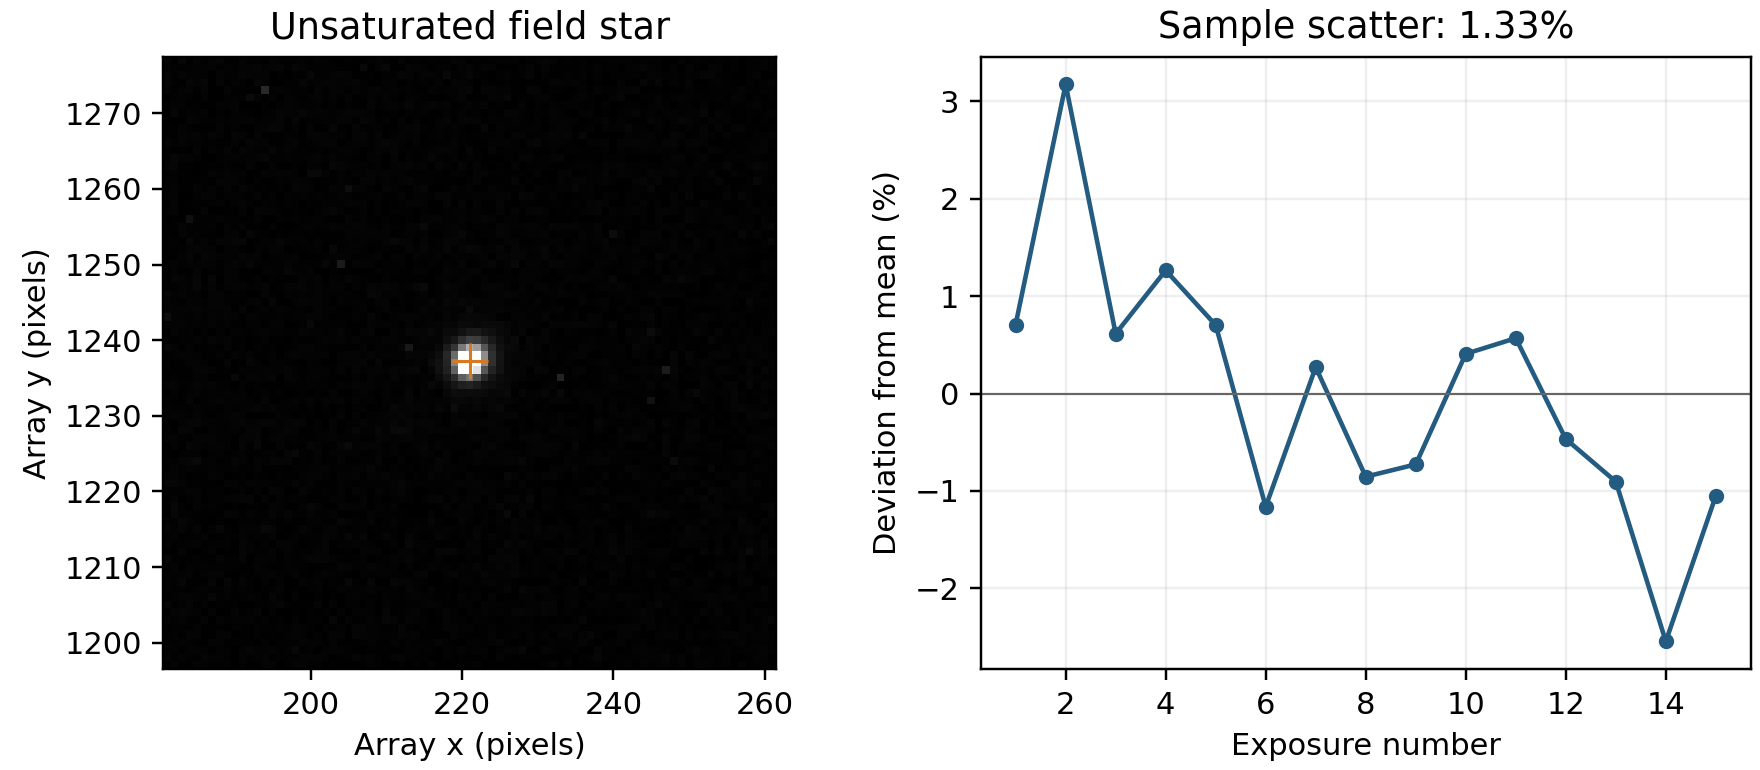
\includegraphics[width=\textwidth]{unsaturated_field_star_check.png}
\caption{Supplementary unsaturated field star in the first calibrated
image (left) and percentage count-rate deviations over 15 images
(right). The marker identifies the measured center. The scatter is
the sample SD divided by the mean; no individual error bars are shown.}
\label{fig:c_field_star}
\end{figure*}

\subsection{Exposure Time, FWHM, and Count Rate}
We measured 12 images spanning 6--300 s with a 30-pixel aperture and
45--75-pixel sky annulus. These files are unbinned
($3056\times3056$ pixels), unlike the $2\times2$ focus and
repeatability sequences. The widths and aperture radii in this
subsection therefore refer to unbinned pixels. FITS headers identify Image 25 as a 150-s
exposure, correcting the original 180-s note.

\begin{table*}[tp]
 \centering
 \caption{Ogma exposure-time measurements using a
 30-pixel photometric aperture. Peak values are the
 reported values from the measurement images; they
 should not be interpreted as a universal raw-detector
 saturation threshold.}
 \label{tab:exposure_measurements}
 \begin{tabular}{crrrr}
  \toprule
  Image & Time (s) & FWHM (pixels) &
  Rate ($\mathrm{DN\,s^{-1}}$) & Peak (DN)\\
  \midrule
  15 & 6   & 6.79  & 297312 & 26361\\
  18 & 8   & 6.64  & 299378 & 41512\\
  17 & 10  & 7.30  & 275574 & 44927\\
  19 & 12  & 7.83  & 242015 & 44972\\
  16 & 15  & 8.61  & 237392 & 44877\\
  20 & 20  & 9.22  & 197273 & 45015\\
  21 & 45  & 12.50 & 159497 & 45064\\
  22 & 60  & 14.50 & 158589 & 44998\\
  23 & 90  & 16.36 & 131787 & 45139\\
  24 & 120 & 17.50 & 113424 & 45165\\
  25 & 150 & 17.24 & 87429  & 45385\\
  26 & 300 & 22.97 & 69921  & 45897\\
  \bottomrule
 \end{tabular}
\end{table*}

FWHM increased from 6.79 pixels at 6 s to 22.97 pixels at 300 s.
Long images also became elongated. For a stable, unsaturated point
source, exposure time alone should not broaden the profile. In this
sequence, tracking motion and distortion of the saturated core can
both increase the measured width. Per-image FWHM uncertainties were
unavailable, so the plot has no numerical error bars.

In a linear detector with stable conditions and a fixed enclosed-light
fraction, count rate $R=C_{\mathrm{source-sky}}/t$ should remain
constant. Instead, it fell from about $2.97\times10^5$ and
$2.99\times10^5~\mathrm{DN\,s^{-1}}$ at 6 and 8 s to
$6.99\times10^4~\mathrm{DN\,s^{-1}}$ at 300 s.

\begin{figure*}[htbp]
 \centering
 \reportfigure[width=0.8\textwidth]
 {ogma_count_rate_vs_exposure.pdf}
 \caption{Background-subtracted Ogma count rate versus
 exposure time, measured with a 30-pixel aperture.
 The measured rate decreases at longer exposures.}
 \label{fig:count_rate_exposure}
\end{figure*}

Nonlinearity and aperture losses are plausible causes of the decline;
transparency changes and calibration residuals may also contribute.
Individual count errors were unavailable for this series.

\subsubsection{Aperture Test}
For Images 21--26, we compared 17- and 30-pixel apertures, with sky
annuli of 34--67 and 45--75 pixels, respectively.

\begin{table*}[tp]
 \centering
 \caption{Ogma count rates measured with 17-pixel
 and 30-pixel aperture radii.}
 \label{tab:aperture_comparison}
 \begin{tabular}{rrrr}
  \toprule
  Time (s) & 17 pixels ($\mathrm{DN\,s^{-1}}$) &
  30 pixels ($\mathrm{DN\,s^{-1}}$) & Increase (\%)\\
  \midrule
  45  & 153936 & 159497 & 3.6\\
  60  & 152043 & 158589 & 4.3\\
  90  & 125309 & 131787 & 5.2\\
  120 & 107010 & 113424 & 6.0\\
  150 & 82187  & 87429  & 6.4\\
  300 & 63712  & 69921  & 9.7\\
  \bottomrule
 \end{tabular}
\end{table*}

The larger aperture recovered 3.6--9.7\% more signal, with the greatest
increase at 300 s. This supports some loss of light from the smaller
aperture as the profile broadened, although changing the sky annulus
also affects the comparison. The larger aperture did not remove the
count-rate decline, so aperture size alone does not explain it.

\subsection{Saturated Profiles}
The exposure-series peak rose from 26361 DN at 6 s to 41512 DN at
8 s, then stayed near 45000 DN from about 10 s onward.

\begin{figure}[htbp]
 \centering
 \reportfigure[width=0.9\linewidth]{ogma_300s_image.png}
 \vspace{3pt}
 \reportfigure[width=\linewidth]
 {Ogma Stellar Profile 6s.png}

 \vspace{0.15cm}

 \reportfigure[width=\linewidth]
 {Ogma Stellar Profile 300s.png}
 \caption{Original 300-s Ogma image cutout (top), followed by
 the retained 6-s and 300-s intensity profiles. The image shows
 elongation; the profiles use the measurement-image signal scale.
 The short exposure has a narrow,
 rounded peak; the long exposure shows a broad,
 flattened core near 45000 DN, consistent with
 saturation or nonlinear response.}
 \label{fig:saturation_profiles}
\end{figure}

The flat core indicates lost flux and a distorted FWHM, while the
elongation shows motion during the exposure. The 45000-DN plateau,
49000-DN repeatability peaks, and dome-flat limit use different
processing or detector settings and do not define one common
saturation threshold.

% Allow pending figures to flow across exercise boundaries.
\section{Exercise D: Color Photometry}
\subsection{Observations and Stellar Measurements}
We observed the open cluster M29 and reflection nebula NGC 7129
through B, V, and R filters. M29 has fifteen 30-s images per filter,
for 450 s of integration in each band. The nebula pipeline combines
15 exposures per filter.

For M29, we measured the same stars in the three aligned stacks with
AstroImageJ's Multi-Aperture tool, using an 8-pixel aperture and
15--22-pixel sky annulus. We selected 12 stars, then excluded Stars
10 and 11 because their R-band peaks were near the apparent saturation
level. Ten stars remain in the color analysis
(Figure~\ref{fig:m29_finding_chart}).

We prepared separate master dome flats for B, V, and R and used
AstroImageJ's Data Processor to divide the science images by the
corresponding normalized flat. The saved R-band setup applies the master bias and
\texttt{Dome\_Flat\_R\_Master.fit}, with dark subtraction disabled.
The master-flat combination method was not recorded. We aligned and averaged
the calibrated science exposures within each filter to produce the
three stacks used for photometry.

\begin{figure}[htbp]
    \centering
    \reportfigure[width=0.9\linewidth]
    {M29_labels.png}
 \caption{M29 field showing the 12 stars selected
    for aperture photometry in AstroImageJ. The
    numbered apertures correspond to the stars
    measured in the B, V, and R filters. Stars
    10 and 11 were excluded from the final
    color-color analysis because of possible
    saturation in the R-band image.}
    \label{fig:m29_finding_chart}
\end{figure}

\subsection{Instrumental Colors and Errors}
Instrumental magnitude is
\begin{equation}
m_{\mathrm{inst}}=-2.5\log_{10}(C/t),
\end{equation}
where $C$ is the background-subtracted signal in an averaged stack.
Each stack averages fifteen 30-s exposures, so it retains the mean
single-exposure signal scale and uses $t=30$ s, despite a total
integration of 450 s per band. This common normalization cancels
in the color ratios:
\begin{align}
(B-V)_{\mathrm{inst}}&=-2.5\log_{10}(C_B/C_V),\\
(V-R)_{\mathrm{inst}}&=-2.5\log_{10}(C_V/C_R).
\end{align}
We propagated AstroImageJ's source-count errors through
\begin{equation}
\sigma_m=\frac{2.5}{\ln10}\frac{\sigma_C}{C}
\end{equation}
and, assuming independent errors between filters,
\begin{align}
\sigma_{B-V}&=\sqrt{\sigma_B^2+\sigma_V^2},\\
\sigma_{V-R}&=\sqrt{\sigma_V^2+\sigma_R^2}.
\end{align}
The colors share V, giving
$\operatorname{Cov}(B-V,V-R)=-\sigma_V^2$.
Horizontal and vertical bars show marginal errors, not this covariance.
They also exclude calibration and atmospheric systematics; their
accuracy depends on the stack's noise model.

\subsection{M29 Results}
Python calculated colors and propagated errors from the AstroImageJ
export. Table~\ref{tab:m29_counts} lists the signals in B, V, R order;
Table~\ref{tab:m29_colors} gives the instrumental colors.

\begin{table*}[tp]
\centering
\caption{Background-subtracted M29 signals and formal AstroImageJ uncertainties in DN, rounded to the nearest DN.}
\label{tab:m29_counts}
\begin{tabular}{crrr}
\toprule
Star & B (DN) & V (DN) & R (DN) \\
\midrule
1 & $272429 \pm 671$ & $578024 \pm 967$ & $692679 \pm 1019$ \\
2 & $258869 \pm 664$ & $608546 \pm 986$ & $811736 \pm 1079$ \\
3 & $152103 \pm 574$ & $348257 \pm 840$ & $455550 \pm 896$ \\
4 & $231023 \pm 643$ & $521315 \pm 942$ & $681979 \pm 1019$ \\
5 & $160092 \pm 582$ & $367103 \pm 853$ & $467630 \pm 904$ \\
6 & $205532 \pm 619$ & $548129 \pm 951$ & $731946 \pm 1037$ \\
7 & $119655 \pm 550$ & $252116 \pm 787$ & $300119 \pm 808$ \\
8 & $76431 \pm 504$ & $312512 \pm 819$ & $529038 \pm 934$ \\
9 & $175259 \pm 594$ & $478265 \pm 915$ & $679195 \pm 1012$ \\
12 & $256088 \pm 657$ & $602996 \pm 978$ & $756523 \pm 1046$ \\
\bottomrule
\end{tabular}
\end{table*}

\begin{table}[htbp]
    \centering
    \caption{Instrumental color indices of the
    10 selected stars in the M29 field.}
    \label{tab:m29_colors}
    \begin{tabular}{ccc}
        \toprule
        Star & $B-V$ (mag) & $V-R$ (mag) \\
        \midrule
        1  & $0.817 \pm 0.003$ & $0.196 \pm 0.002$ \\
        2  & $0.928 \pm 0.003$ & $0.313 \pm 0.002$ \\
        3  & $0.899 \pm 0.005$ & $0.292 \pm 0.003$ \\
        4  & $0.884 \pm 0.004$ & $0.292 \pm 0.003$ \\
        5  & $0.901 \pm 0.005$ & $0.263 \pm 0.003$ \\
        6  & $1.065 \pm 0.004$ & $0.314 \pm 0.002$ \\
        7  & $0.809 \pm 0.006$ & $0.189 \pm 0.004$ \\
        8  & $1.529 \pm 0.008$ & $0.572 \pm 0.003$ \\
        9  & $1.090 \pm 0.004$ & $0.381 \pm 0.003$ \\
        12 & $0.930 \pm 0.003$ & $0.246 \pm 0.002$ \\
        \bottomrule
    \end{tabular}
\end{table}

\begin{figure*}[tp]
    \centering
    \reportfigure[width=\textwidth]
    {m29_color_color.pdf}
 \caption{Instrumental color-color diagram
    for 10 stars in the M29 field. Each point
    is labeled with its corresponding star
    number. The left panel contains all ten stars; the right enlarges
    the central group, with Star 8 outside that view. Error bars
    represent propagated formal photometric uncertainties.}
    \label{fig:m29_color_color}
\end{figure*}

The two colors show a positive association: stars with larger B--V
usually also have larger V--R. Most B--V values lie between 0.81 and
1.09 mag. Star 8 is relatively redder, with
$B-V=1.529\pm0.008$ mag and $V-R=0.572\pm0.003$ mag.
It follows the color trend and was retained.

Stellar color depends on surface temperature, while interstellar dust
can redden the observed light \cite{colors,dust}. Thus Star 8 could
differ in temperature or reddening, or be a field star rather than an
M29 member. Our measurements cannot distinguish those explanations.
We have not applied standard-system zero points or color transformations,
so the instrumental indices do not directly yield temperatures or
spectral types.

\subsection{NGC 7129 Composite}
For the nebula, the Python pipeline in
\nolinkurl{D_NGC7129.ipynb} constructed and applied separate
dome flats for B, V, and R. It retained 18 B flats, 15 V flats, and 20 R flats, excluding
B frames 9 and 19 and V frames 4, 6, 8, 16, and 20. We normalized
each retained flat by its median, median-combined each filter's flats,
and renormalized the masters to unity.

The science inputs were recorded as already dark-corrected. We
removed the 100-DN stored pedestal by adding the signed
\texttt{PEDESTAL=-100} value, then divided by the matching flat:
\begin{equation}
I_{\mathrm{corrected}}=I_{\mathrm{science}}/F_{\mathrm{normalized}}.
\end{equation}
No additional bias or dark subtraction was applied. Python aligned
the calibrated images to the first V image using \texttt{astroalign},
then median-combined the 15 exposures in each band.

The initial composite had a strong greenish-blue background gradient.
We estimated each filter's background with a $31\times31$-pixel
median filter followed by Gaussian smoothing ($\sigma=120$ pixels),
then subtracted the model:
\begin{equation}
I_{\mathrm{final}}(x,y)=I_{\mathrm{corrected}}(x,y)-B(x,y).
\end{equation}
For display, we subtracted each channel's median, clipped negative
values to zero, scaled by the 99.5th percentile, and applied an
inverse hyperbolic sine stretch. R, V, and B map to red, green,
and blue, respectively.

\begin{figure}[htbp]
    \centering
    \reportfigure[width=0.85\linewidth]
    {NGC7129_background_corrected.png}
 \caption{Final BVR color composite
    of NGC 7129 after dome-flat correction,
    alignment, stacking, and large-scale
    background subtraction. The image is slightly cropped to remove edge artifacts.}
    \label{fig:ngc7129_final}
\end{figure}

The composite shows the reflection nebula against a more uniform
background. Independent channel scaling makes its color qualitative.
The smoothed background model may also remove faint extended
nebulosity, so we do not use this image for surface-brightness or
quantitative color measurements.

\subsection{Improvements}
For M29, the formal photometric errors should account for the noise
reduction from averaging 15 frames. Standard stars would allow
transformation to a standard photometric system; membership information
would help interpret the cluster colors. For NGC 7129, better-matched
flats and a background model that masks both stars and nebulosity
would improve illumination correction while preserving diffuse structure.
Additional exposures would improve sensitivity to faint emission.

% Allow pending figures to flow across exercise boundaries.
\section{Exercise E: Plate Scale}
\subsection{Observations and Component Identification}
On September 24, we observed ten double-star targets, primarily
through the [O III] filter, using $2\times2$ binning and
$1528\times1528$-pixel images. Most targets had three 30-s exposures;
HR6446 also had additional 60-s exposures. Figure~\ref{fig:e_plan}
records the original AstroPlanner target list. Its separations are
planning values; the calculations below use the WDS measurements
and years explicitly listed in Table~\ref{tab:e_verified} \cite{wds}.

\begin{figure*}[tp]
\centering
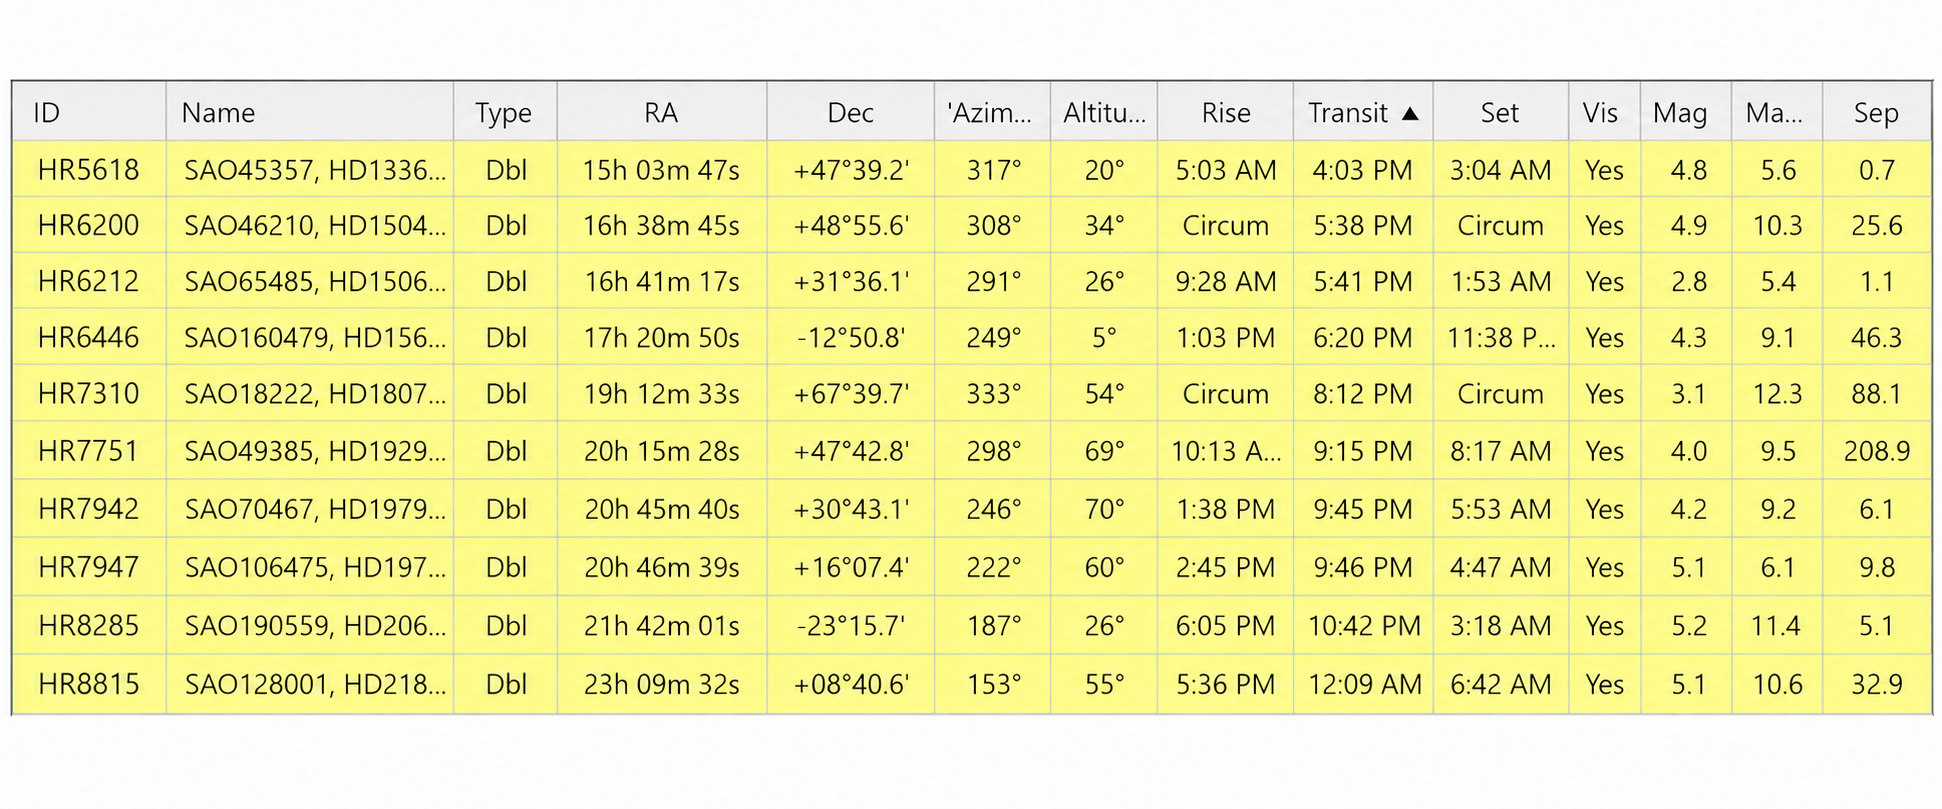
\includegraphics[width=\textwidth]{observing-plan-unhighlighted.png}
\caption{Original AstroPlanner observing plan for the ten targets.
The listed separations are distinct from the later WDS reference
values used in our calculations.}
\label{fig:e_plan}
\end{figure*}

We identified HR6200, HR7751, HR8815, and HR7310 by matching their
fields to DSS2 red survey images from CDS \cite{dss}. Affine fits to
27, 33, 13, and 22 surrounding stars gave RMS residuals of
1.8, 1.3, 1.4, and 1.2 arcseconds, respectively. Companion directions
agreed with the catalog. These checks establish the field orientation
and component selection; saturated survey primaries prevent precise
new binary astrometry.

\begin{figure*}[p]
\centering
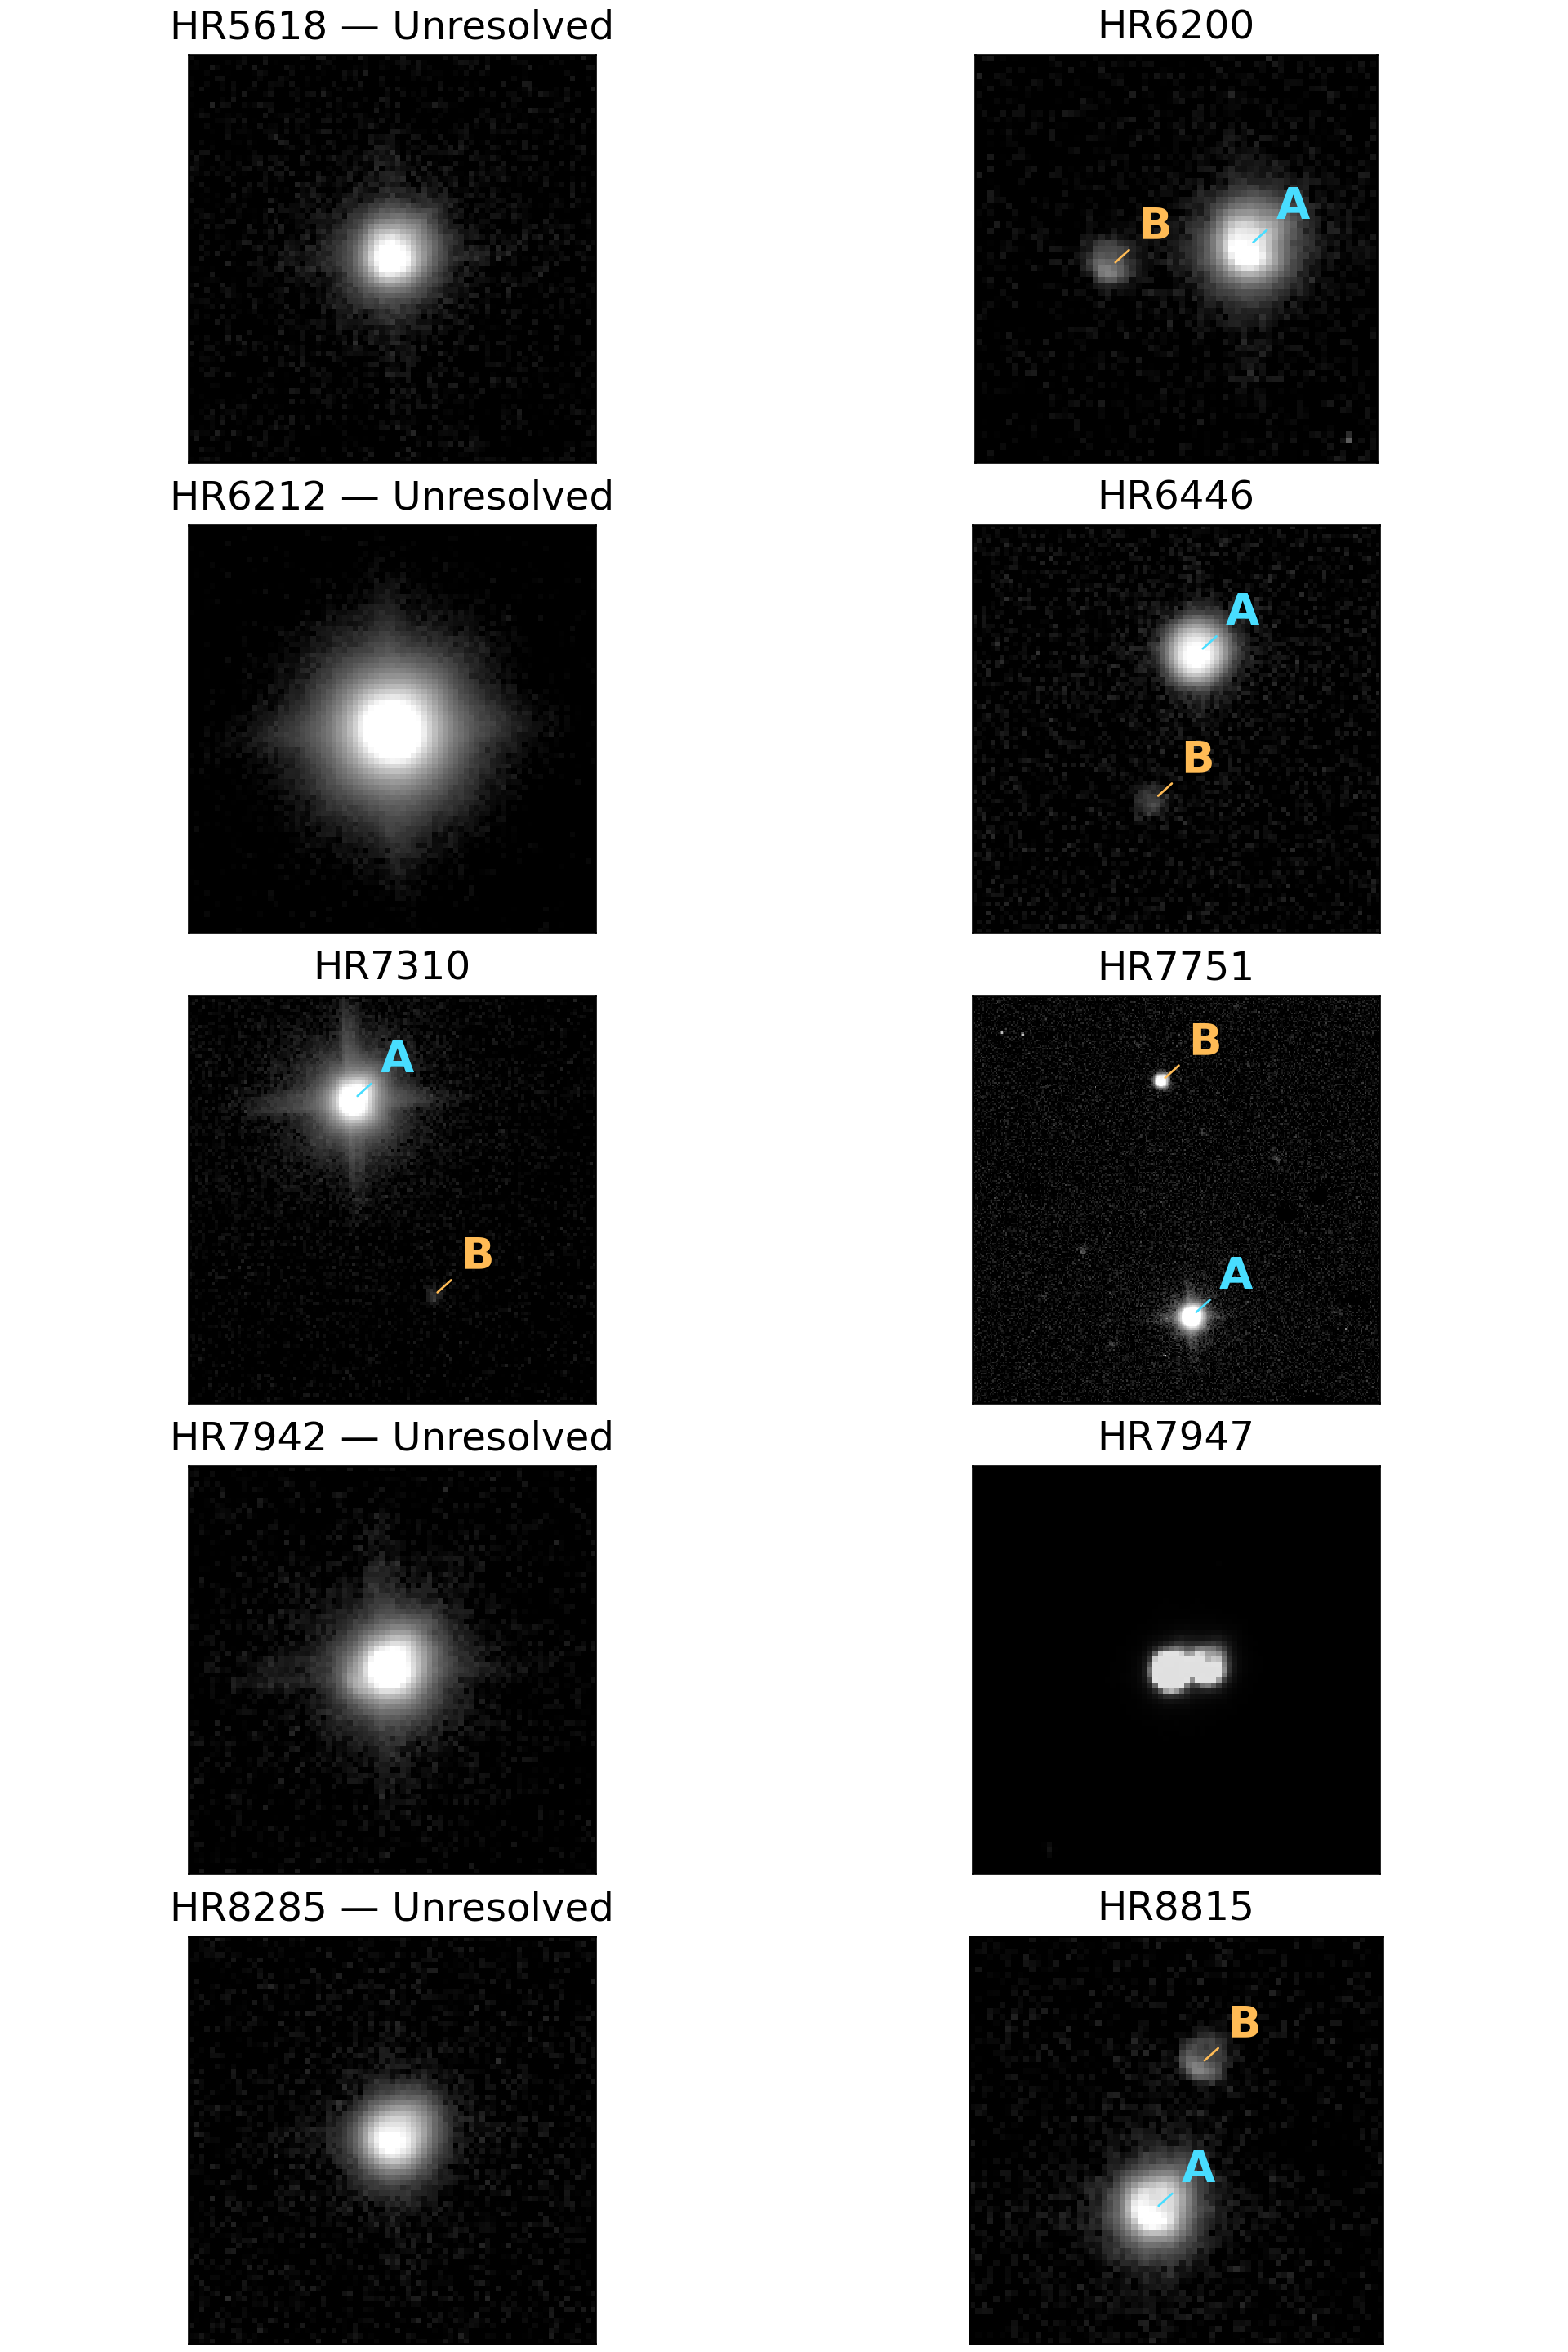
\includegraphics[width=\textwidth,height=0.84\textheight,keepaspectratio]{E_observed_fields.png}
\caption{Close-ups of the ten observed double-star fields. A and B
mark the measured components of verified pairs and the HR6446
candidate. Unconfirmed targets are shown without companion labels.
Panels use different crops and display stretches. HR7310 uses its
full signal range, and HR7947 uses a linear display to show the two
overlapping cores. The panels follow FITS array orientation, not a
common celestial orientation.}
\label{fig:e_observed_fields}
\end{figure*}

\subsection{Repeated Measurements and Plate Scale}
We measured HR6200, HR7751, and HR8815 in three exposures each
with AstroImageJ. HR6200 and HR8815 used 9-pixel primary and
4-pixel companion apertures with 40--60-pixel sky annuli. HR7751
used 6-pixel apertures and 19--26-pixel annuli. Both components have
positive net signals in these measurements.

For HR7310, supplementary Python measurements used a
background-subtracted 12-pixel-radius centroid for the primary and
a robust Gaussian plus planar-background fit to the companion in a
$17\times17$-pixel box. The faint companion peaks at 308--355 DN.
These measurements replace the earlier selection of a different
field star.

For each exposure, we calculated
\begin{align}
d&=\sqrt{(x_2-x_1)^2+(y_2-y_1)^2},\\
p&=\theta/d,
\end{align}
where $d$ is the binned-pixel separation and $\theta$ is the angular
separation of the same WDS pair. Table~\ref{tab:e_verified} reports
the mean of the three individual scales for each target. The
accompanying \nolinkurl{E_verified_repeats.csv} contains the centroids.

\begin{table*}[tp]
\centering
\caption{Verified binary measurements. Uncertainties in mean pixel
distance and mean plate scale are SEMs of three exposures; they
exclude catalog and shared systematic errors.}
\label{tab:e_verified}
\begin{tabular}{lrrrr}
\toprule
Target & \makecell{WDS separation\\(arcsec; year)} &
\makecell{Individual distances\\(pixels)} &
\makecell{Mean distance\\(pixels)} &
\makecell{Mean scale\\(arcsec pixel$^{-1}$)}\\
\midrule
HR6200 & 28.1; 2020 & 22.557, 22.791, 22.746 & $22.698\pm0.072$ & $1.2380\pm0.0039$\\
HR7751 & 208.5; 2015 & 166.458, 166.340, 166.492 & $166.430\pm0.046$ & $1.2528\pm0.0003$\\
HR8815 & 32.6; 2015 & 25.422, 25.490, 25.306 & $25.406\pm0.054$ & $1.2832\pm0.0027$\\
HR7310 & 80.4; 2021 & 65.050, 65.406, 65.404 & $65.287\pm0.118$ & $1.2315\pm0.0022$\\
\bottomrule
\end{tabular}
\end{table*}

The four pair means span 1.232--1.283 arcseconds per pixel, more
than their repeat SEMs can explain. Giving each binary equal weight,
we obtain
\begin{equation}
\boxed{\bar p=1.251\pm0.012~\mathrm{arcsec\,pixel^{-1}}}.
\end{equation}
The sample SD is $0.023~\mathrm{arcsec\,pixel^{-1}}$; the quoted
SEM is this value divided by $\sqrt{4}$. It assumes independent
between-target errors. The WDS summary gives no separation errors,
and the catalog epochs differ. Catalog motion, centroid bias,
nonlinearity, and field distortion are not fully included. Four
pairs are insufficient to map distortion across the detector.

\begin{figure*}[tp]
\centering
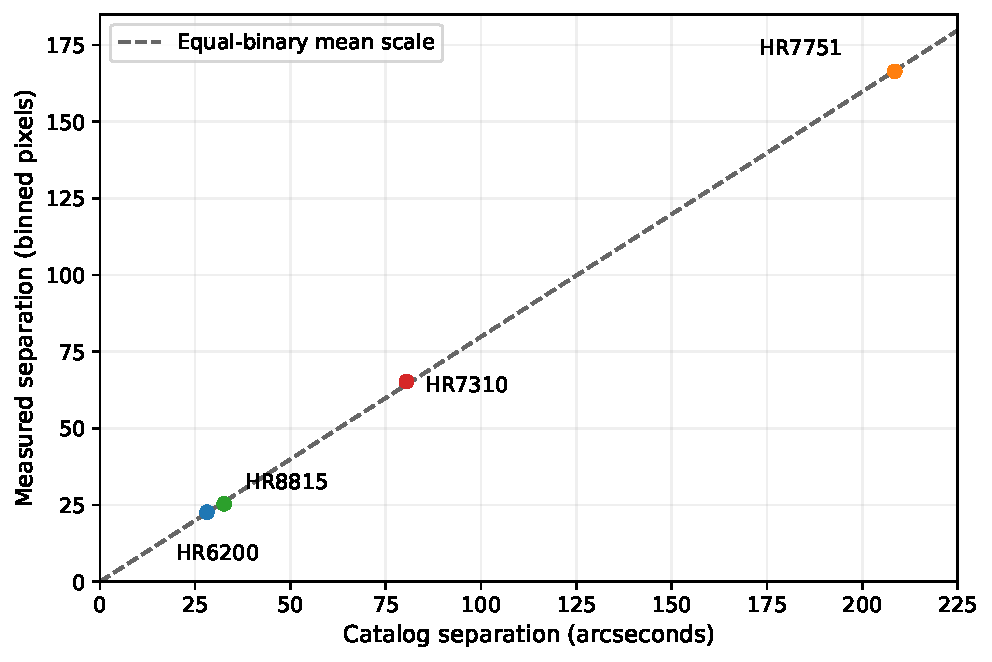
\includegraphics[width=0.8\textwidth]{E_separation_pixels_vs_arcsec.pdf}
\caption{Mean pixel separation versus WDS angular separation for
the four verified binaries. Vertical bars show repeat SEMs and are
smaller than the symbols. The dashed line uses the equal-binary mean
scale, $d=\theta/\bar p$; it is not a weighted regression. Catalog
uncertainties are unavailable and are not represented by the bars.}
\label{fig:e_separation_plot}
\end{figure*}

\subsection{Other Targets and Measurement Limits}
Four of the ten targets gave usable calibration measurements.
HR5618 was unresolved. HR7947 shows two overlapping bright cores,
but reliable separate centroids were not obtained. The selected
components of HR6212, HR7942, and HR8285 remain uncertain.
For HR7310, the corrected AB identification replaces the field star
about 273 arcseconds away. We use the WDS separation of 80.4
arcseconds (2021), rather than AstroPlanner's older 88.1-arcsecond
planning value.

HR6446's visible candidate companion gave inconsistent separations:
34.335 and 35.774 pixels with the same supplementary fitting method.
The third exposure was excluded because of a streak or image artifact.
We excluded HR6446 from the calibration because its identification
and centering remain uncertain.

The initial AstroImageJ angular distances encode a common scale
setting of $0.1109116~\mathrm{arcsec\,pixel^{-1}}$. We used the
measured pixel coordinates and independent catalog separations
instead.

\subsection{Angular Image Width and Field of View}
The faint components of HR6200 and HR8815 have low peaks
(1273--1702 DN) and provide six unsaturated width measurements in
three exposures of each field. Their AstroImageJ FWHMs average
3.471 pixels, with a sample SD of 0.318 pixels. Applying
$w=\bar p\,\mathrm{FWHM}_{\mathrm{pix}}$ gives a characteristic
angular image width of
\begin{equation}
\boxed{w\simeq4.34~\mathrm{arcsec}}.
\end{equation}
The between-image and between-star width scatter corresponds to
0.40 arcsecond (sample SD); the scale SEM contributes another
0.05 arcsecond to the mean width. Focus, tracking, and sampling also broaden the images, so this is
an observed image width rather than a pure atmospheric seeing value.

At the same $2\times2$ binning,
\begin{equation}
\mathrm{FOV}=\frac{\bar p\,1528}{60}
\times\frac{\bar p\,1528}{60},
\end{equation}
so the nominal full-array field is
\begin{equation}
\boxed{\mathrm{FOV}\simeq31.87\times31.87~\mathrm{arcmin}}.
\end{equation}
Each side has an empirical scale contribution of 0.29 arcminute
from the adopted SEM; the two side uncertainties are fully correlated.
This estimate excludes distortion and any cropped image borders.

\section*{Conclusion}
The CCD read noise was $10.045\pm0.007$ DN, and the gain at
$2\times2$ binning was $1.290\pm0.006~\mathrm{e^-\,DN^{-1}}$.
Dark charge increased with exposure time and temperature. The
apparent activation energy was $0.95\pm0.14$ eV, limited by the
unmatched bias and uncertain detector temperatures.

Best focus was near $16000~\mu\mathrm{m}$. Saturated Ogma images
showed 6.86\% count-rate scatter; an unsaturated field star in the
same sequence showed 1.33\%. Longer exposures broadened and lost
measured count rate, consistent with tracking and saturation effects
and some aperture loss.

M29 showed a spread of instrumental colors, with Star 8 the reddest
of the retained sample. The NGC 7129 composite revealed the nebula,
although its display colors and faint background are not calibrated.
Four visual binaries gave a plate scale of
$1.251\pm0.012~\mathrm{arcsec\,pixel^{-1}}$ and a nominal
$31.87\times31.87$-arcminute field. Unsaturated companions had a mean
angular image width of 4.34 arcseconds with 0.40-arcsecond sample
scatter. Better temperature records, unsaturated exposures, and more
binary measurements would improve the main results.

\begin{thebibliography}{9}
\bibitem{manual}
ASTRO 320W, \textit{Observing Exercise Manual}, version August 22, 2026.
\bibitem{progress4}
Davis, G., Artemis Group, \textit{Observing Progress Report 4},
September 24, 2026, pp.~1--2.
\bibitem{camera}
Diffraction Limited, \textit{SBIG STX and STXL Large Format CCD Detectors},
technical specifications, December 2019.
\url{https://cdn.diffractionlimited.com/downloads/STX-STXLOverview.pdf}
\bibitem{wds}
U.S. Naval Observatory, \textit{Washington Double Star Catalog},
summary tables for 12--17 h and 18--23 h, accessed October 20, 2026.
\url{https://www.astro.gsu.edu/wds/}
\bibitem{dss}
Space Telescope Science Institute / CDS, \textit{Digitized Sky Survey 2,
red survey}, accessed through the CDS HiPS2FITS service,
October 20, 2026.
\url{https://alasky.cds.unistra.fr/hips-image-services/hips2fits}
\bibitem{colors}
OpenStax, \textit{Astronomy 2e}, Section 17.2, ``Colors of Stars.''
\url{https://openstax.org/books/astronomy-2e/pages/17-2-colors-of-stars}
\bibitem{dust}
OpenStax, \textit{Astronomy 2e}, Section 20.3, ``Cosmic Dust.''
\url{https://openstax.org/books/astronomy-2e/pages/20-3-cosmic-dust}
\end{thebibliography}

\clearpage
\onecolumn
\appendix
\titleformat{\section}{\large\bfseries}{Appendix \thesection:}{0.5em}{}
\section{Analysis Code}
The accompanying repository contains the executed notebooks in
\nolinkurl{notebooks/}, measurement exports in \nolinkurl{data/},
and the original gain workbook in \nolinkurl{spreadsheets/}.
The two \nolinkurl{A320_bf_stdev} algorithms were supplied by the
instructor. Original C and D routines and supplementary analyses
are identified in the notebook introductions. The compact listing
below summarizes the main numerical calculations.

\noindent\textbf{Repository preparation.}
ChatGPT was used to help organize and clean the repository, remove
duplicate and superseded files, convert Python scripts to Jupyter
notebooks, and revise the repository documentation.

\lstinputlisting[language=Python,linewidth=\linewidth,
 xleftmargin=5pt,xrightmargin=5pt,framesep=4pt]{report_calculations_listing.txt}
\end{document}
